% !TEX root=../main.tex

\chapter{ICARUS-T600 detector operations and event reconstruction}
\label{chap:event_reconstruction}

The ICARUS detector, described in \autoref{sec:ICARUS_T600} is a complex system, and a precise operation is required to make the most out of all its subcomponents. Each part of the online operation is essential and preliminary to the offline operations, consisting of the wireplane signal processing, the reconstruction of all the signals coming from the different subsystems and their combination to obtain a final physics result. 

\section{Data acquisition} \label{sec:DAQ}


\paragraph{ICARUS trigger} The ICARUS trigger employs the coincidence between the signal from the beams (BNB and NuMI) spill gates with the scintillation light to provide a global signal that activates  the acquisition windows for the TPC and PMT subsystems. For TPC, the acquisition window is driven by the time it takes for drift electrons to cross half of each T300 module: with a nominal electric drift field of \SI{500}{\volt\per\cm}, and a half-width of $\sim\SI{1.5}{\m}$, the drift time is chosen to be $\SI{1.6}{\ms}$. The acquisition window for PMTs is driven by the mean lifetime of LAr excited states. De-excitation of LAr produces scintillation light in two components, one fast $\tau\simeq \SI{6}{\ns}$ and one slow $\tau\simeq\SI{1.6}{\us}$. To collect the full scintillation light, the time window has to be thus greater than \SI{1.6}{\us}. Additionally, in the case of a second light trigger in the \SI{10}{\us} immediate subsequent window --- this could be the case for a cosmic-induced muon crossing the detector during the drifting of the electrons ---, the readout is extended by \SI{7}{\us}. Finally, a \SI{7}{\us} buffer before the global trigger is also kept, adding up to a total of \SI{26}{\us} of PMT acquisition window.  

The ICARUS trigger architecture allows for multiple configurations, i.e. the acquisition of different types of events \cite{ICARUS:2025kai}, with and without beam (on- and off-beam), and requiring or not requiring the PMT light signal (majority or minimum bias). The main ICARUS trigger physics configuration (on-beam majority) is based on the multiplicity of PMT signals in coincidence with the beam ``open'' spill gate. Off-beam cosmic ray events are collected with similar ``off-beam majority'', requiring the coincidence between the light signal and off-beam gates, generated \SI{33}{\ms} after on-beam gates. Minimum bias (both for on- and off-beam configurations) triggers are generated in the presence of the corresponding gate, regardless of the presence of scintillation light.

\paragraph{Collection of the triggered events. } Once a global trigger is present, the data acquisition system (DAQ), which communicates via TCP/IP protocol with the trigger system, activates the readout of the whole detector, with \SI{1.6}{\ms} and \SI{26}{\us} for the TPC and PMTs, respectively. ICARUS DAQ is based on the \emph{artdaq} data acquisition software development kit developed at Fermilab \cite{Biery:2013cda}. The \emph{artdaq} SDK provides  customisable applications for reading data fragments from detector elements, which are identified as \emph{BoardReader} objects in the \emph{artdaq} language, and configurable applications for performing event-building (i.e. merging together the collected data fragments from each \emph{BordReader}, performed by objects inherited from \emph{EventBuilder} instances), data-logging and data-dispatch to downstream online data quality monitoring processes. 

Customised \emph{BoardReaders} acquire data fragments from all ICARUS subdetectors, TPC, PMT and CRT readout electronics, and from trigger and White Rabbit: this latter subsystem, not described in \autoref{sec:ICARUS_T600}, is a CERN-developed technology that provides global timing across all subdetectors and serves also as a double check against trigger global timing. Event counters and timestamps are assigned accordingly to each data fragment, which are then queued for data transfer to a configurable number of \emph{EventBuilder} instances. When an event is triggered, the corresponding trigger \emph{BoardReader} instance sends the trigger data fragment to the \emph{EventBuilder}. This triggers a request for data from all other configured \emph{BoardReader}s in the DAQ system. \autoref{fig:DAQ} shows a simplified illustration of the DAQ working principle. 

\begin{figure}
    \centering
    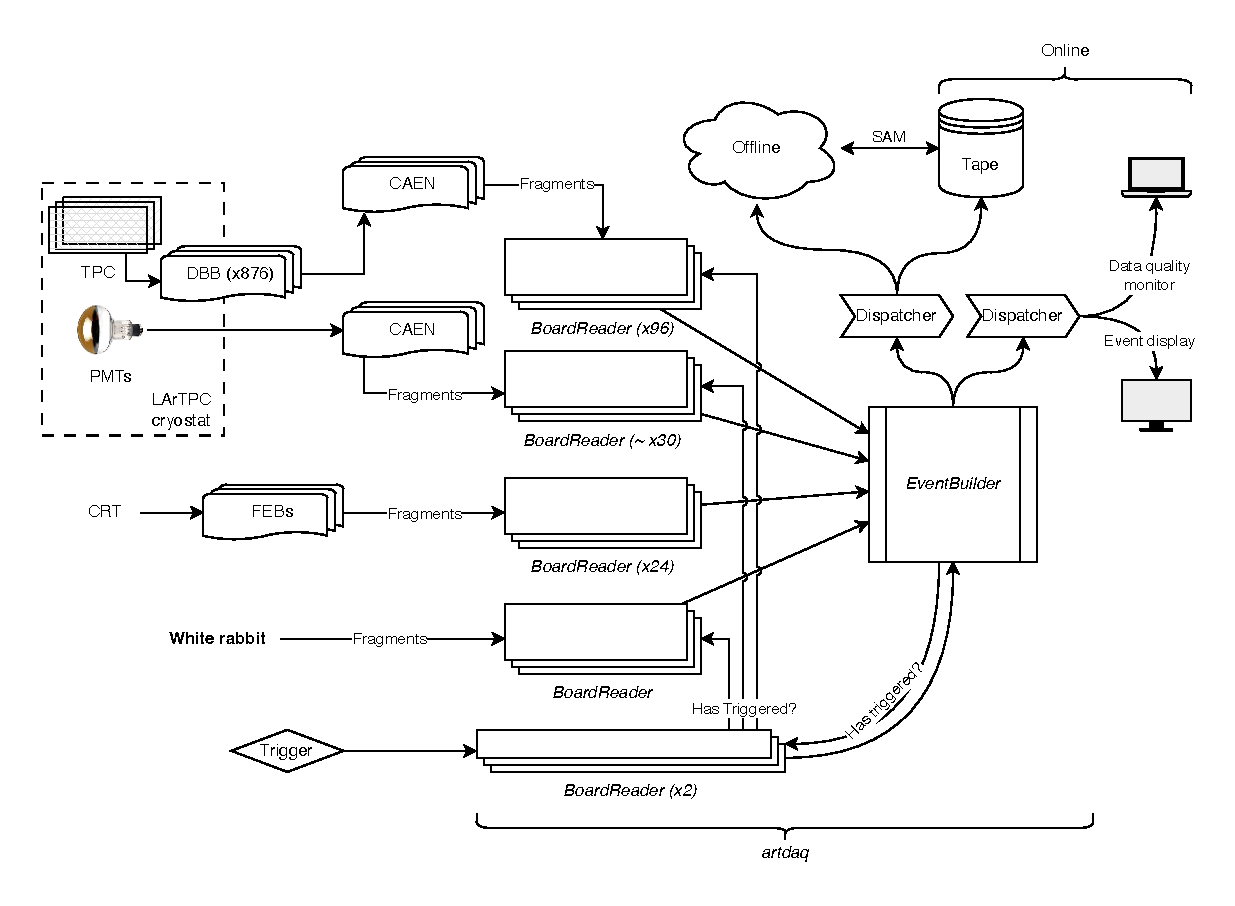
\includegraphics[width=\linewidth]{detector/DAQ_simplified.pdf}
    \caption[ICARUS DAQ illustration]{Simplified illustration of the ICARUS DAQ system. Further information is found in \autoref{sec:DAQ}. The number of parallel \emph{EventBuilder} instances could be defined $\geq1$, to allow for faster processing.}
    \label{fig:DAQ}
\end{figure}

The data collected by the ICARUS DAQ system is written in different file streams depending on which beam it is detecting and which trigger configuration is active, whether on- or off-beam, minimum bias or majority. 

Downstream of the DAQ interface, events are written using the \emph{art} event-processing framework \cite{greenArtFramework2012} also developed at Fermilab, on which the \emph{artdaq} SDK is built. This allows flawless interoperability between the DAQ interface and the offline analysis, without the need to convert the events saved from the DAQ interface into a format compatible with the high-level offline analysis. After a long testing and commissioning phase, the DAQ system was reported to be able to stably handle high data rates up to \SI{5}{\hertz}. This is, however, well in excess of what the detector is supposed to be handling, given the BNB and NuMI data rates when using a majority-based trigger configuration, based on light scintillation, delivering about \SI{1}{\hertz} of data throughput.  

In order to handle the large volumes of data stored on tape, the Fermilab-based SAM (serial access to metadata) system is exploited. This system associates a set of metadata information with each data file using Python scripts. This metadata is useful in offline analysis to create large datasets of files, identifying whether the files contain raw or processed data, run configuration, run number and so on.

\section{ICARUS data processing}

The output data files contain the aggregated data coming from all the \emph{BoardReader} instances in an event. For the TPC, the data correspond to the digitised waveforms from each TPC readout channel, representing the charge induced by the motion of ionisation electrons drifted by the electric field inside the detector. Similarly, the data from the PMTs correspond to the digitised waveforms of the readout of every PMT inside the detector, corresponding of the scintillation light deposited in each PMT. For the CRT system the DAQ process is slightly different \cite{ICARUS:2025rdw,Poppi:2023zmp,Poppi:2022vhg}. The ICARUS CRTs operate in self-trigger mode \cite{arteroponsStudyReconstructionNuMuCC, ICARUS:2025rdw}, whenever a CRT SiPM exceeds the threshold, the data from all 32 SiPM channels for each FEB is stored in internal buffers, holding up to \qtyrange{40}{80}{\ms} depending on which CRT sub-part is considered. The data from the top, bottom and side CRTs is aggregated within \SI{10}{\us} data fragments in the \emph{BoardReader}s instances; once the global trigger is activated, \SI{+-25}{\ms} of CRT data fragments are sent from the \emph{BoardReader} to the \emph{EventBuilder} instance. 

The output of all ICARUS sub-detectors is common across LArTPC detectors, which might have different TPC geometry and light collection configurations but share the same underlying technology. The \emph{art}-based \emph{LArSoft} framework \cite{Church:2013hea,Snider:2017wjd,Pordes:2017BL} is the common software development kit providing software infrastructure and algorithms for simulation of Monte Carlo data, processing of both simulated and real data, and event reconstruction. The key to \emph{LArSoft} is the use of real-time configuration files that employ the \emph{Fermilab Hierarchical Configuration Language}, or \emph{FHiCL}, which specify how different modules of the processing chain should be run. 

When an event is saved from DAQ to data files and stored to tape, it is then available to be processed. The ICARUS data processing chain is split, like for many other LArTPC detectors, into two \emph{stages}, usually named \emph{Stage0} or \emph{reco1} and \emph{Stage1} or \emph{reco2}. Processing the raw collected data is a mandatory step in order for it to be properly analysed. 

In the \emph{Stage0/reco1} step, all data  from the three sub-detectors is processed to produce a ``simpler'' description of the raw signal. This means to decode the raw signal and translate it into objects in the \emph{LArSoft} format for offline reconstruction. It also performs signal processing of the waveforms to identify physical signals, hits, that can then be used as input to the higher-level event reconstruction tools implemented in the \emph{Stage1/reco2} steps. 

\begin{figure}
    \centering
    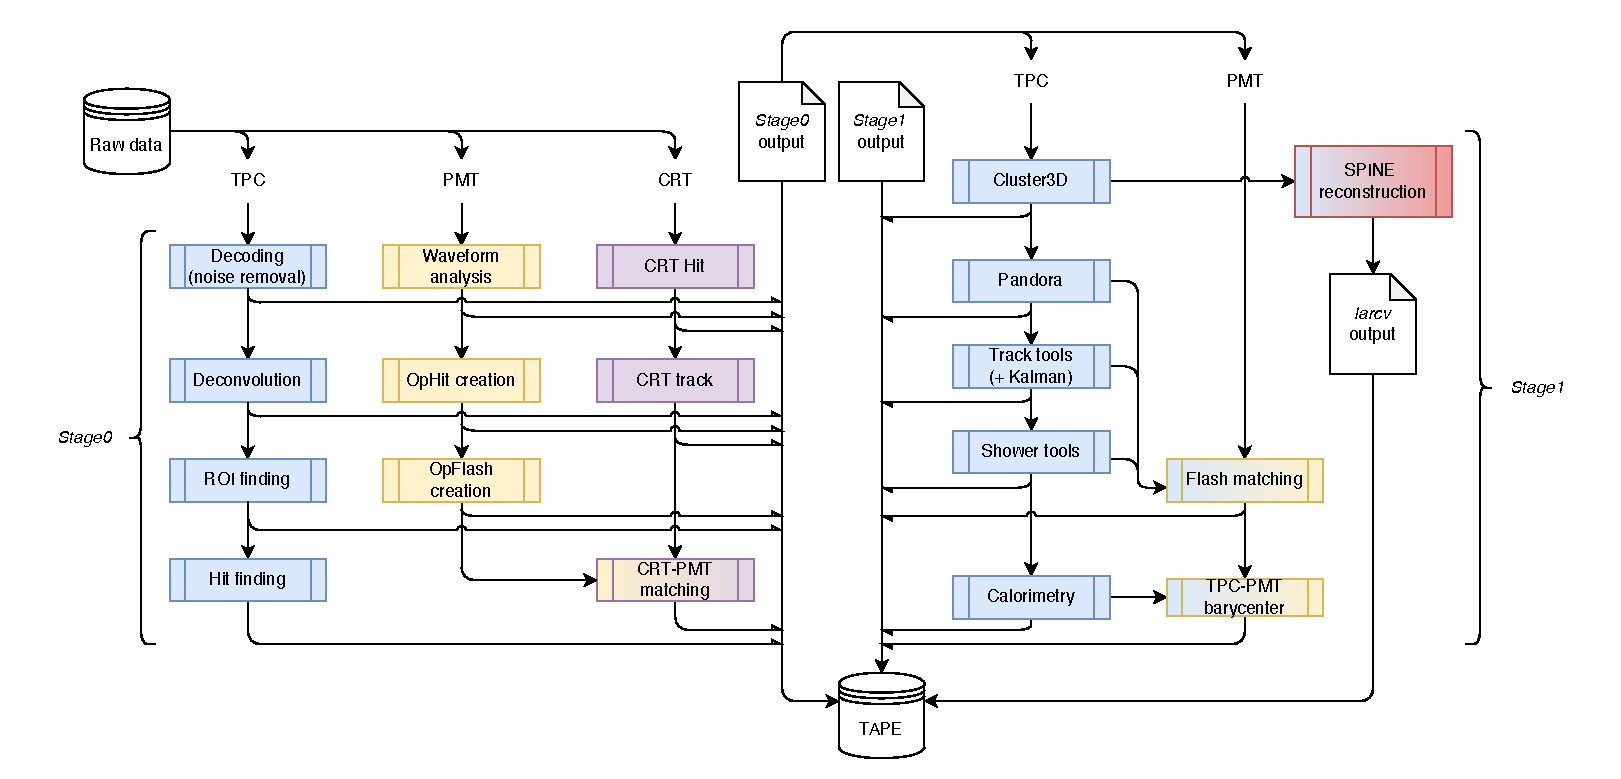
\includegraphics[width=\linewidth]{detector/data_processing_pipeline.pdf}
    \caption[\emph{Stage0} and \emph{Stage1} data processing pipeline]{Illustration of the data processing pipeline used in the ICARUS detector showing the steps involved in both \emph{Stage0} and \emph{Stage1}. }
    \label{fig:reco_stages}
\end{figure}

\autoref{fig:reco_stages} pictures the overall \emph{Stage0/Stage1} chain which is applied to the data files produced by the ICARUS DAQ. A detailed description of these steps follows in the next paragraphs. 

\section{Light reconstruction}

One of the first steps in \emph{Stage0} reconstruction addresses the reconstruction of the light signal. Reconstruction of the light signal associated with the event of interest is based on the recorded PMT signals in the events, sampled at \SI{500}{\mega\hertz}. For any event triggered in coincidence with the beam spill, the digitised signals of all 360 PMTs are recorded in \SI{30}{\us} long time intervals. In addition to this data, whenever an off-time cosmic ray event crosses the volume, triggering scintillation light acquired by the PMTs in the \SI{+-1}{\ms} around the beam gate, all 180 PMTs belonging to the T300 module containing the interaction are recorded in \SI{10}{\us} long time intervals. 

The first step in the light reconstruction is the identification of the PMT signal, using a threshold-based approach. To do so, a ``baseline'' has to be defined, which is performed by a sliding window. The pedestal (the \emph{baseline}) is used to then identify the signal over the threshold, using three thresholds defining the start, tail and end points of the PMT hit, called \emph{OpHit}. The algorithm identifies an \emph{OpHit} as the ensemble of these three values and some information about the integral collected charge of the PMT, which is proportional to the light collected. If a start threshold is reached before the end of a previoud \emph{OpHit} the hit is truncated. \autoref{fig:PMT_reco}a shows the example of a PMT with a clear single \emph{OpHit}. 

After individual optical hits are reconstructed, they are clustered together into higher-level objects, called \emph{OpFlash}, corresponding to multiple optical hits happening in proximity inside the detector, hence corresponding to the same physical event inside the volume. \autoref{fig:PMT_reco}b shows multiple PMTs whose \emph{OpHit} are going to be clustered into a single \emph{OpFlash}, corresponding to collected light produced by a single interaction inside the detector. 

All data products created in the \emph{Stage0} PMT processing are saved using the same \emph{LArSoft}-based structure to \emph{ROOT} \cite{rene_brun_2019_3895860} files. 

\begin{figure}
    \centering
    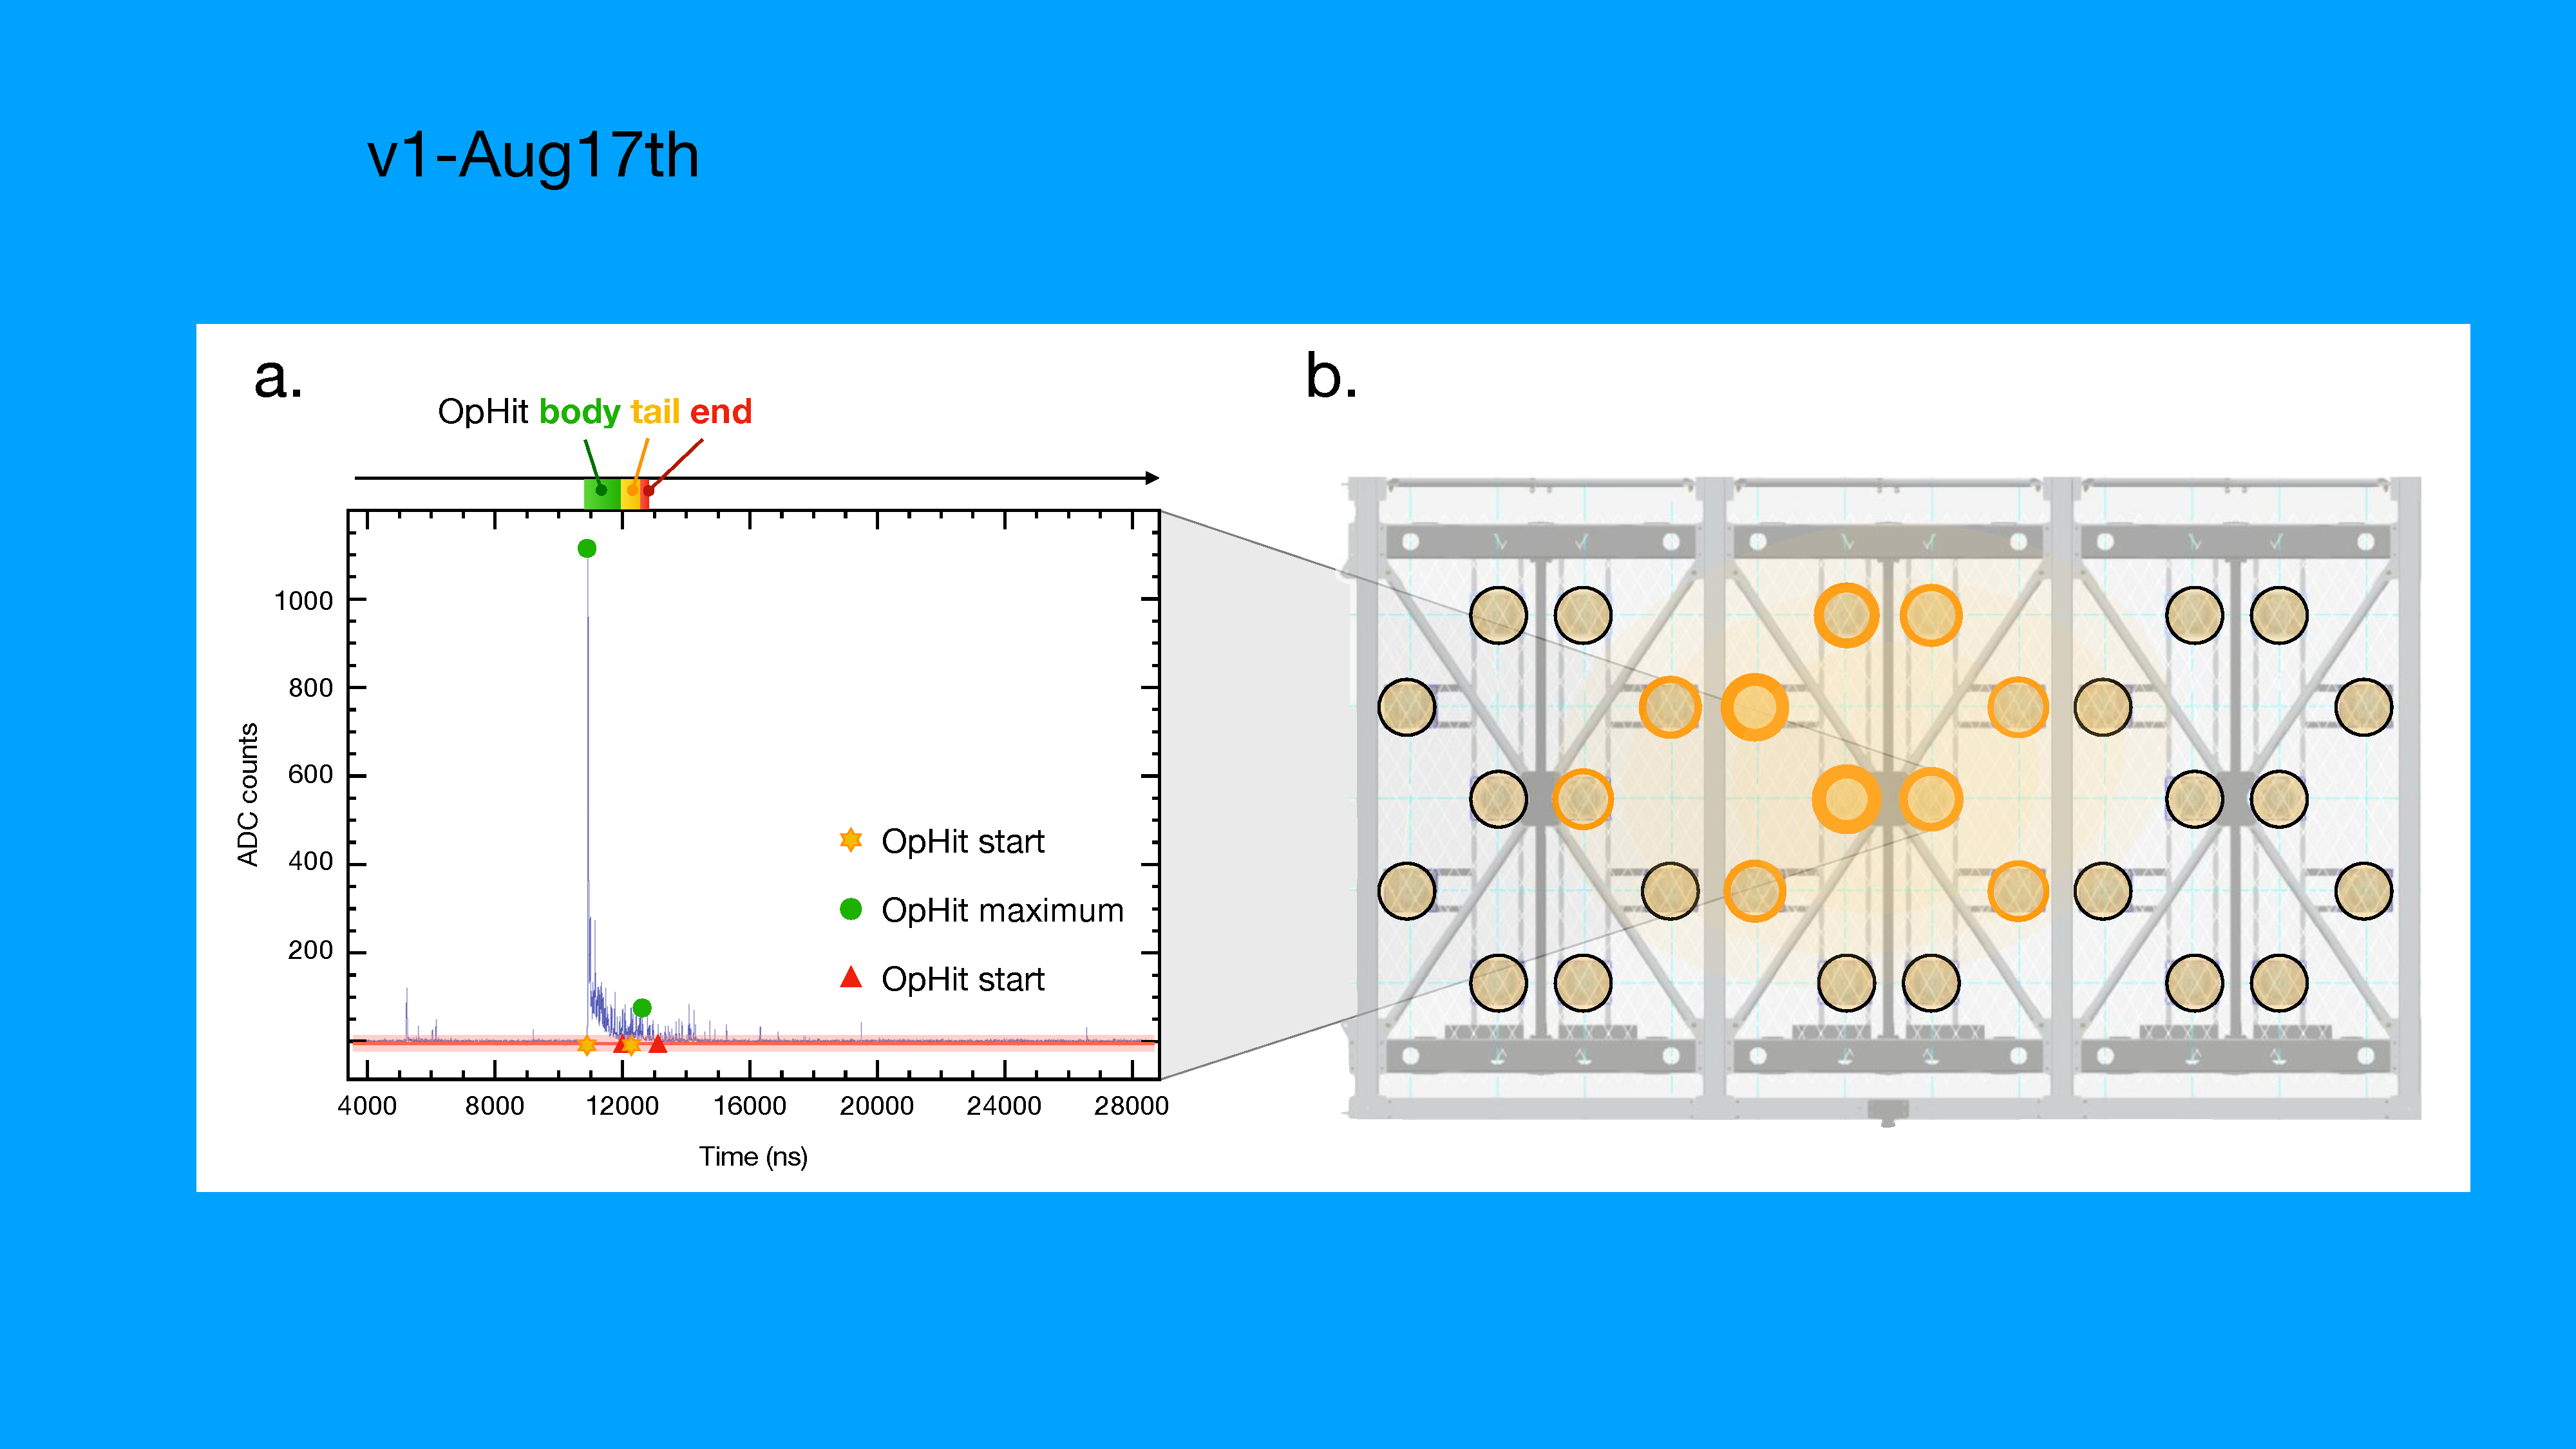
\includegraphics[width=\linewidth,trim={5.5cm 7cm 3.5cm 9cm},clip]{detector/PMT_reco.pdf}
    \caption[PMT reconstructed \emph{OpHits}]{Illustration of an interaction as seen by the PMTs inside the detector volume. (a) shows the pedestal-subtracted waveform produced by a single fired PMT, with the \emph{OpHit} information is clearly marked on top, with the three regions (body, tail and end) highlighted. (b) shows all the PMTs activated during an event in the TPC volume; the PMTs which are over threshold, coloured yellow, will constitute the \emph{OpFlash} object.}
    \label{fig:PMT_reco}
\end{figure}

\section{Wireplanes signal reconstruction}

After the PMT data has been processed, it is time for the TPC wire data. The wire data is the waveform readout of the \num{53248} individual wires, with coherent noise removed by the readout cards. Only minimal further processing is performed online, which leaves more scope for reprocessing the raw data using improved signal processing tools. The recorded waveforms are in ADC count/tick units, where the amplitude of the signal is expressed in ADC counts and the time information in ticks, each corresponding to \SI{0.4}{\us} in the ICARUS TPC timing. \autoref{fig:TPC_signal} shows a sample of the data collected by the three planes, exhibiting the characteristic bipolar shape for the two induction wire planes and a unipolar signal for the collection plane. 

\begin{figure}
    \centering
    \subfloat[]{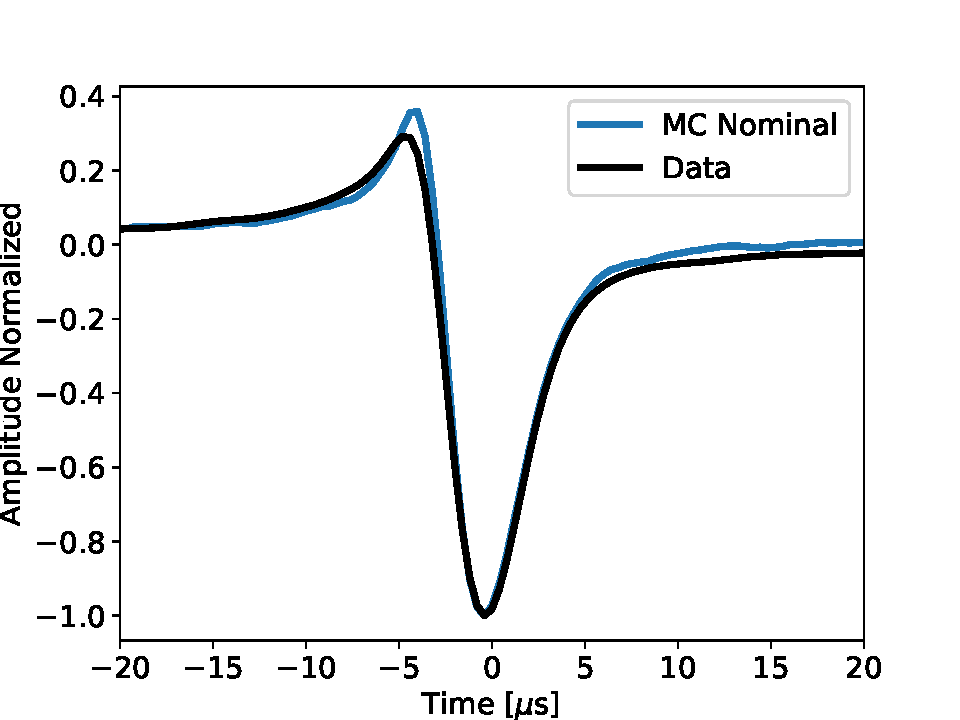
\includegraphics[width=0.3\linewidth]{detector/wvf_data_MCNominal_a20_P0.pdf}\label{fig:TPC_wire_i1}}
    \subfloat[]{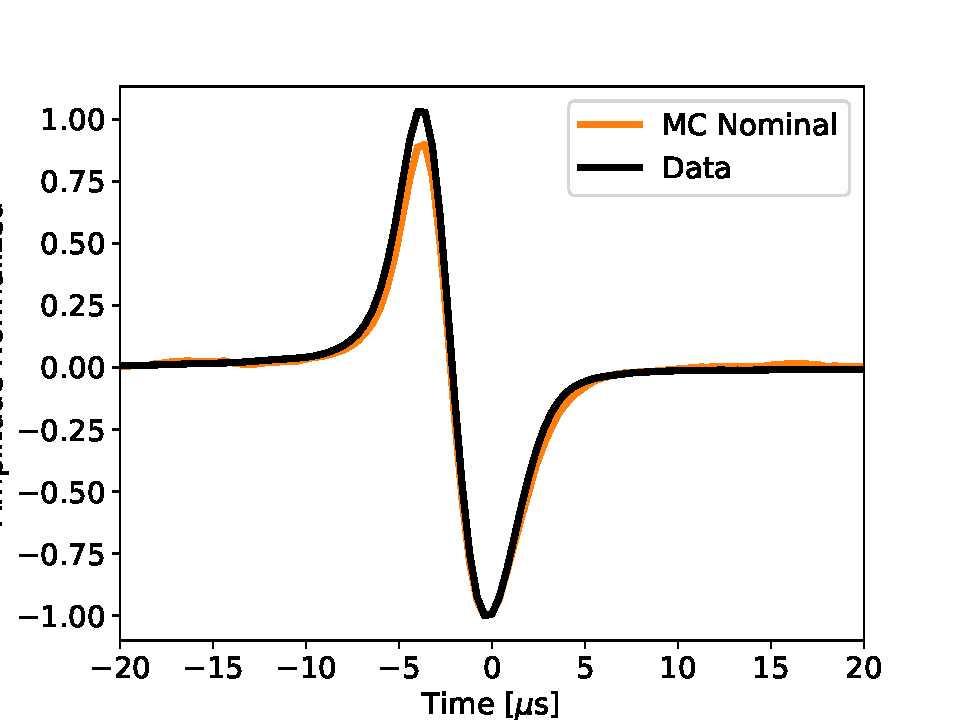
\includegraphics[width=0.3\linewidth]{detector/wvf_data_MCNominal_a20_P1.pdf}\label{fig:TPC_wire_i2}}
    \subfloat[]{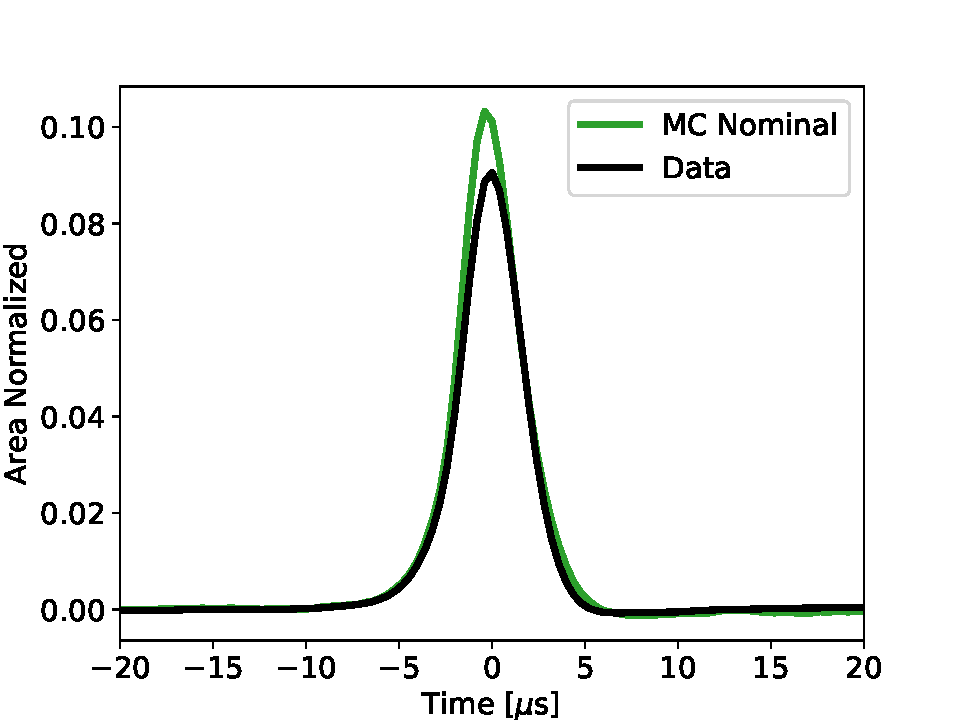
\includegraphics[width=0.3\linewidth]{detector/wvf_data_MCNominal_a20_P2.pdf}\label{fig:TPC_wire_c}}
    \caption[TPC plane signal]{Typical \emph{raw} signal captured by the three planes (induction-1 \ref{sub@fig:TPC_wire_i1}, induction-2 \ref{sub@fig:TPC_wire_i2} and collection \ref{sub@fig:TPC_wire_c}) showing the characteristic bipolar signal for the two induction plane and the unipolar shape for the collection plane. Taken from \cite{ICARUS:2024hmk}. }
    \label{fig:TPC_signal}
\end{figure}

In order to obtain a simplified representation of the information collected by the wireplanes, three major steps are addressed in \emph{Stage0}: \begin{inparaenum}
    \item the wire signals are deconvolved from the TPC electronic response functions, so that all three wire signal are also unipolar in shape;
    \item the signal is analysed in order to define the region-of-interest (ROI) with a threshold-based algorithm; 
    \item each ROI is finally fit using a Gaussian function, whose area is proportional to the number of drift electrons generating the signal. 
\end{inparaenum}

\paragraph{Wire signal processing} The raw decoded wire signal shape is dependent on the distribution of drift electrons, which is core to obtaining calorimetric and particle identification information, but in order to explain such dependency, the raw signal must be processed. The resulting signal $R(t)$ on the wires can be seen as the convolution of serial effects of signal formation, electron propagation, electrostatic field response around the wires and processing by the DAQ to the true electronic signal, so that the response function can be factorised as \begin{equation}
    \begin{aligned}
        R(t, t')&=\mathrm{Ionization\ \otimes\ Recombination\ \otimes\ Diffusion\ and\ Attachment\ \otimes} \\
        &\quad \quad \mathrm{\otimes\ Field\ response\ \otimes\ Electronic\ response\ \otimes\ Electronic\ noise}
    \end{aligned} 
\end{equation} In order to recover the desired ionisation electron yield, useful to have a knowledge of the deposited energy per wire inside the detector as a function of time, it is necessary to unfold these effects. 

The ICARUS detector exploit a signal processing chain similar to other LArTPC experiments, performing a deconvolution in time of the signal waveforms. Ideally, after the deconvolution step, the signal pulse produced by a charged track on the wire would be Gaussian-shaped, with an integral area proportional to the deposited energy inside LAr. The signal recorded on the wires is the convolution of the response function $R$ with the ``true'' $S$ signal, \begin{equation}
    M(t') = \int_{-\infty}^{+\infty} R(t'-t)\ S(t)\ \dd t;
\end{equation} Using the properties of the Fourier transforms, this can be written in the frequency space as $\mathcal M(\omega) = \mathcal R(\omega)\cdot \mathcal S(\omega)$, which can be easily inverted, retrieving the ``true'' signal shape $\mathcal S(\omega)$. This approach, referred to as ``one-dimensional'' deconvolution, is currently employed in most of LArTPC detectors. However, this assumes that the charge distribution on each wire is independent on the charge distribution on the wires in its vicinity. It has been demonstrated that this is not completely true, as can be seen in references \cite{MicroBooNE:2018swd,MicroBooNE:2018vro}. Though it implies small corrections to the overall deposited charge in general, this is not always the case. For example, for isochronous tracks (i.e. tracks lying parallel to the wires, which is somewhat common for the induction-1 wires given the ICARUS geometry), these vicinity effects can create destructive interference patterns.

\begin{figure}
    \centering
    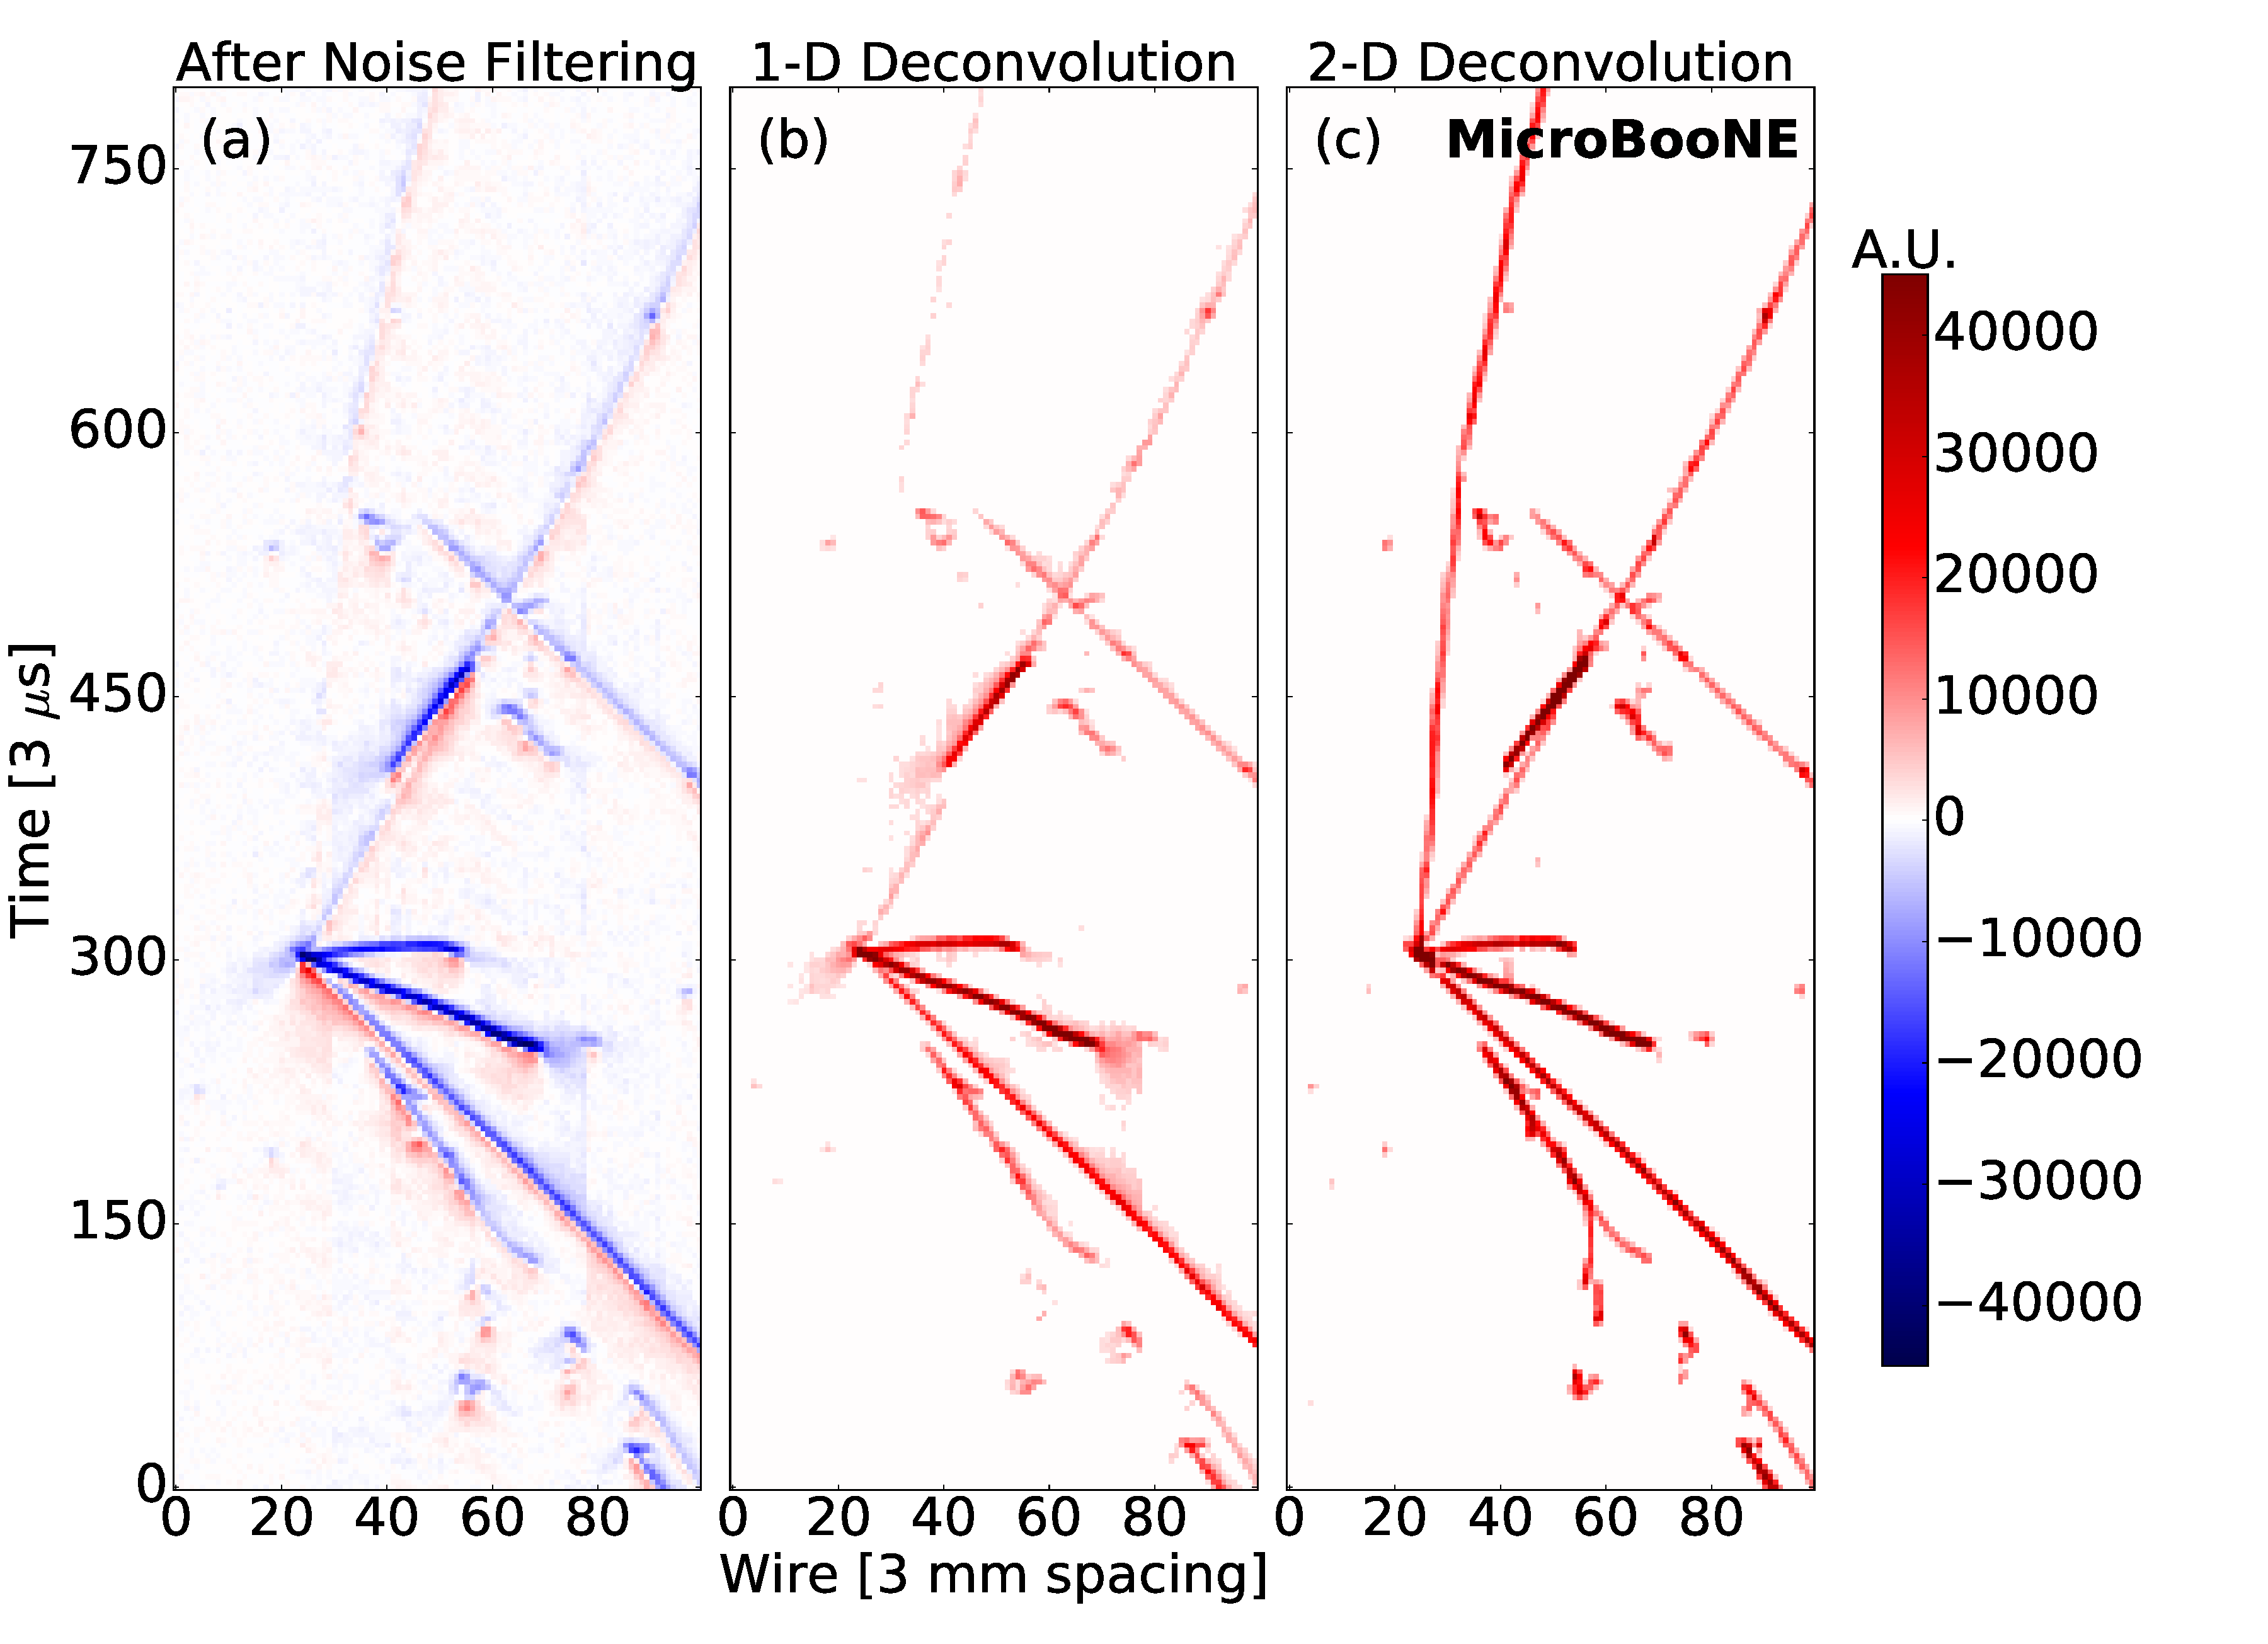
\includegraphics[width=0.85\linewidth]{detector/noiseVs1DVs2D.pdf}
    \caption[TPC signal processing]{Example of the effect of signal processing using the one-dimensional deconvolution approach used in ICARUS (b) with respect to the noise-filtered data (a). (c) shows the same event using a two-dimensional deconvolution approach, performing the deconvolution both in the time direction as well as in the direction of the wires. Taken from \cite{MicroBooNE:2018swd}. }
    \label{fig:uBooNE_signalProc}
\end{figure}

In \cite{MicroBooNE:2018swd,MicroBooNE:2018vro} a solution, adopting two-dimensional deconvolution techniques over both the wire time as well as the wire number, is presented; this provides a strong and computationally efficient method to better extract the distribution of ionisation electrons. \autoref{fig:uBooNE_signalProc} shows the result of the 1D and 2D approaches as tested by the MicroBooNE detector. Tests towards adapting the 2D signal deconvolution are being made inside the ICARUS collaboration, and once validated, should provide a better reconstruction efficiency for the ICARUS TPC detector. 

\paragraph{ROI finding} Once the signal is unipolar in all planes, the next step to define the TPC hits is to select only the ``interesting'' regions of the wires. These regions of interest (ROI) are identified by performing a threshold search in the time domain, allowing to restrict the area on which the hits are created to small portions of the wires. ROIs can be actually relevant to iteratively improve the performances of the 1D/2D deconvolution steps, minimising the time-domain region over which the deconvolution is performed. Once ROIs are identified, a baseline value can be assumed for all other times in the waveform, drastically reducing the size of these data products inside the data files. 

\paragraph{\emph{Hit} creation} Upon the identification of ROIs, the final step is the creation of the \emph{Hit}s objects. A \emph{Hit} is a two-dimensional object representing a cluster of electric drift charges, arriving at a certain time on a certain wire. The hit-finding algorithm runs under the assumption the distribution of the drift charges is Gaussian. Operating on the deconvolved ROI segments of the waveforms, it tries to fit one or multiple Gaussian distributions onto the signal shape. The extracted parameters from the fit process of the Gaussian distribution(s) --- the area, FWHM, the mean, and their multiplicity --- are the properties of the \emph{Hit} objects. The area is proportional to the cumulative charge deposited by the electrons and proportional to the deposited energy inside the detector; the mean and the FWHM represent the hit peak time and its width; the multiplicity can be used to perform operations between adjacent hits. 

At this point, a collection of 2D hits for each plane of wires has been created. The three 2D views of the planes are stored and used as input for the event reconstruction taking place inside \emph{Stage1}. 

\section{Cosmic ray tagger reconstruction} The first step in the reconstruction of the CRT signal is the extraction of the number of photoelectrons $n_\mathrm{p.e.}$ extracted from the ADC count, knowing the amplification gain, subtracting the pedestal \begin{equation}
    n_\mathrm{p.e.} = \frac{\mathrm{\#ADC} - \mathrm{ped}}{G}. 
\end{equation} 

A preliminary selection for the side CRT data is performed, requiring a \SI{7.5}{pe} threshold. The top CRT does not require a preliminary selection based on a threshold but instead requires a quadruple coincidence to generate a hit (see \autoref{fig:CRT_reco}a). At this point it is possible to create the CRT \emph{Hit} objects for side and top CRTs. To each hit object are associated two timestamps:  $T_0$ identifying the global timing of the recorded hit, provided by the White Rabbit switch system, and $T_1$ which identifies the relative timing of the hit with respect to the trigger. Additionally, the CRT hits contain the position in the ICARUS detector frame of reference. Due to the differences in the CRT modules between side and top CRT, the position computation is slightly different. 

\begin{figure}
    \centering
    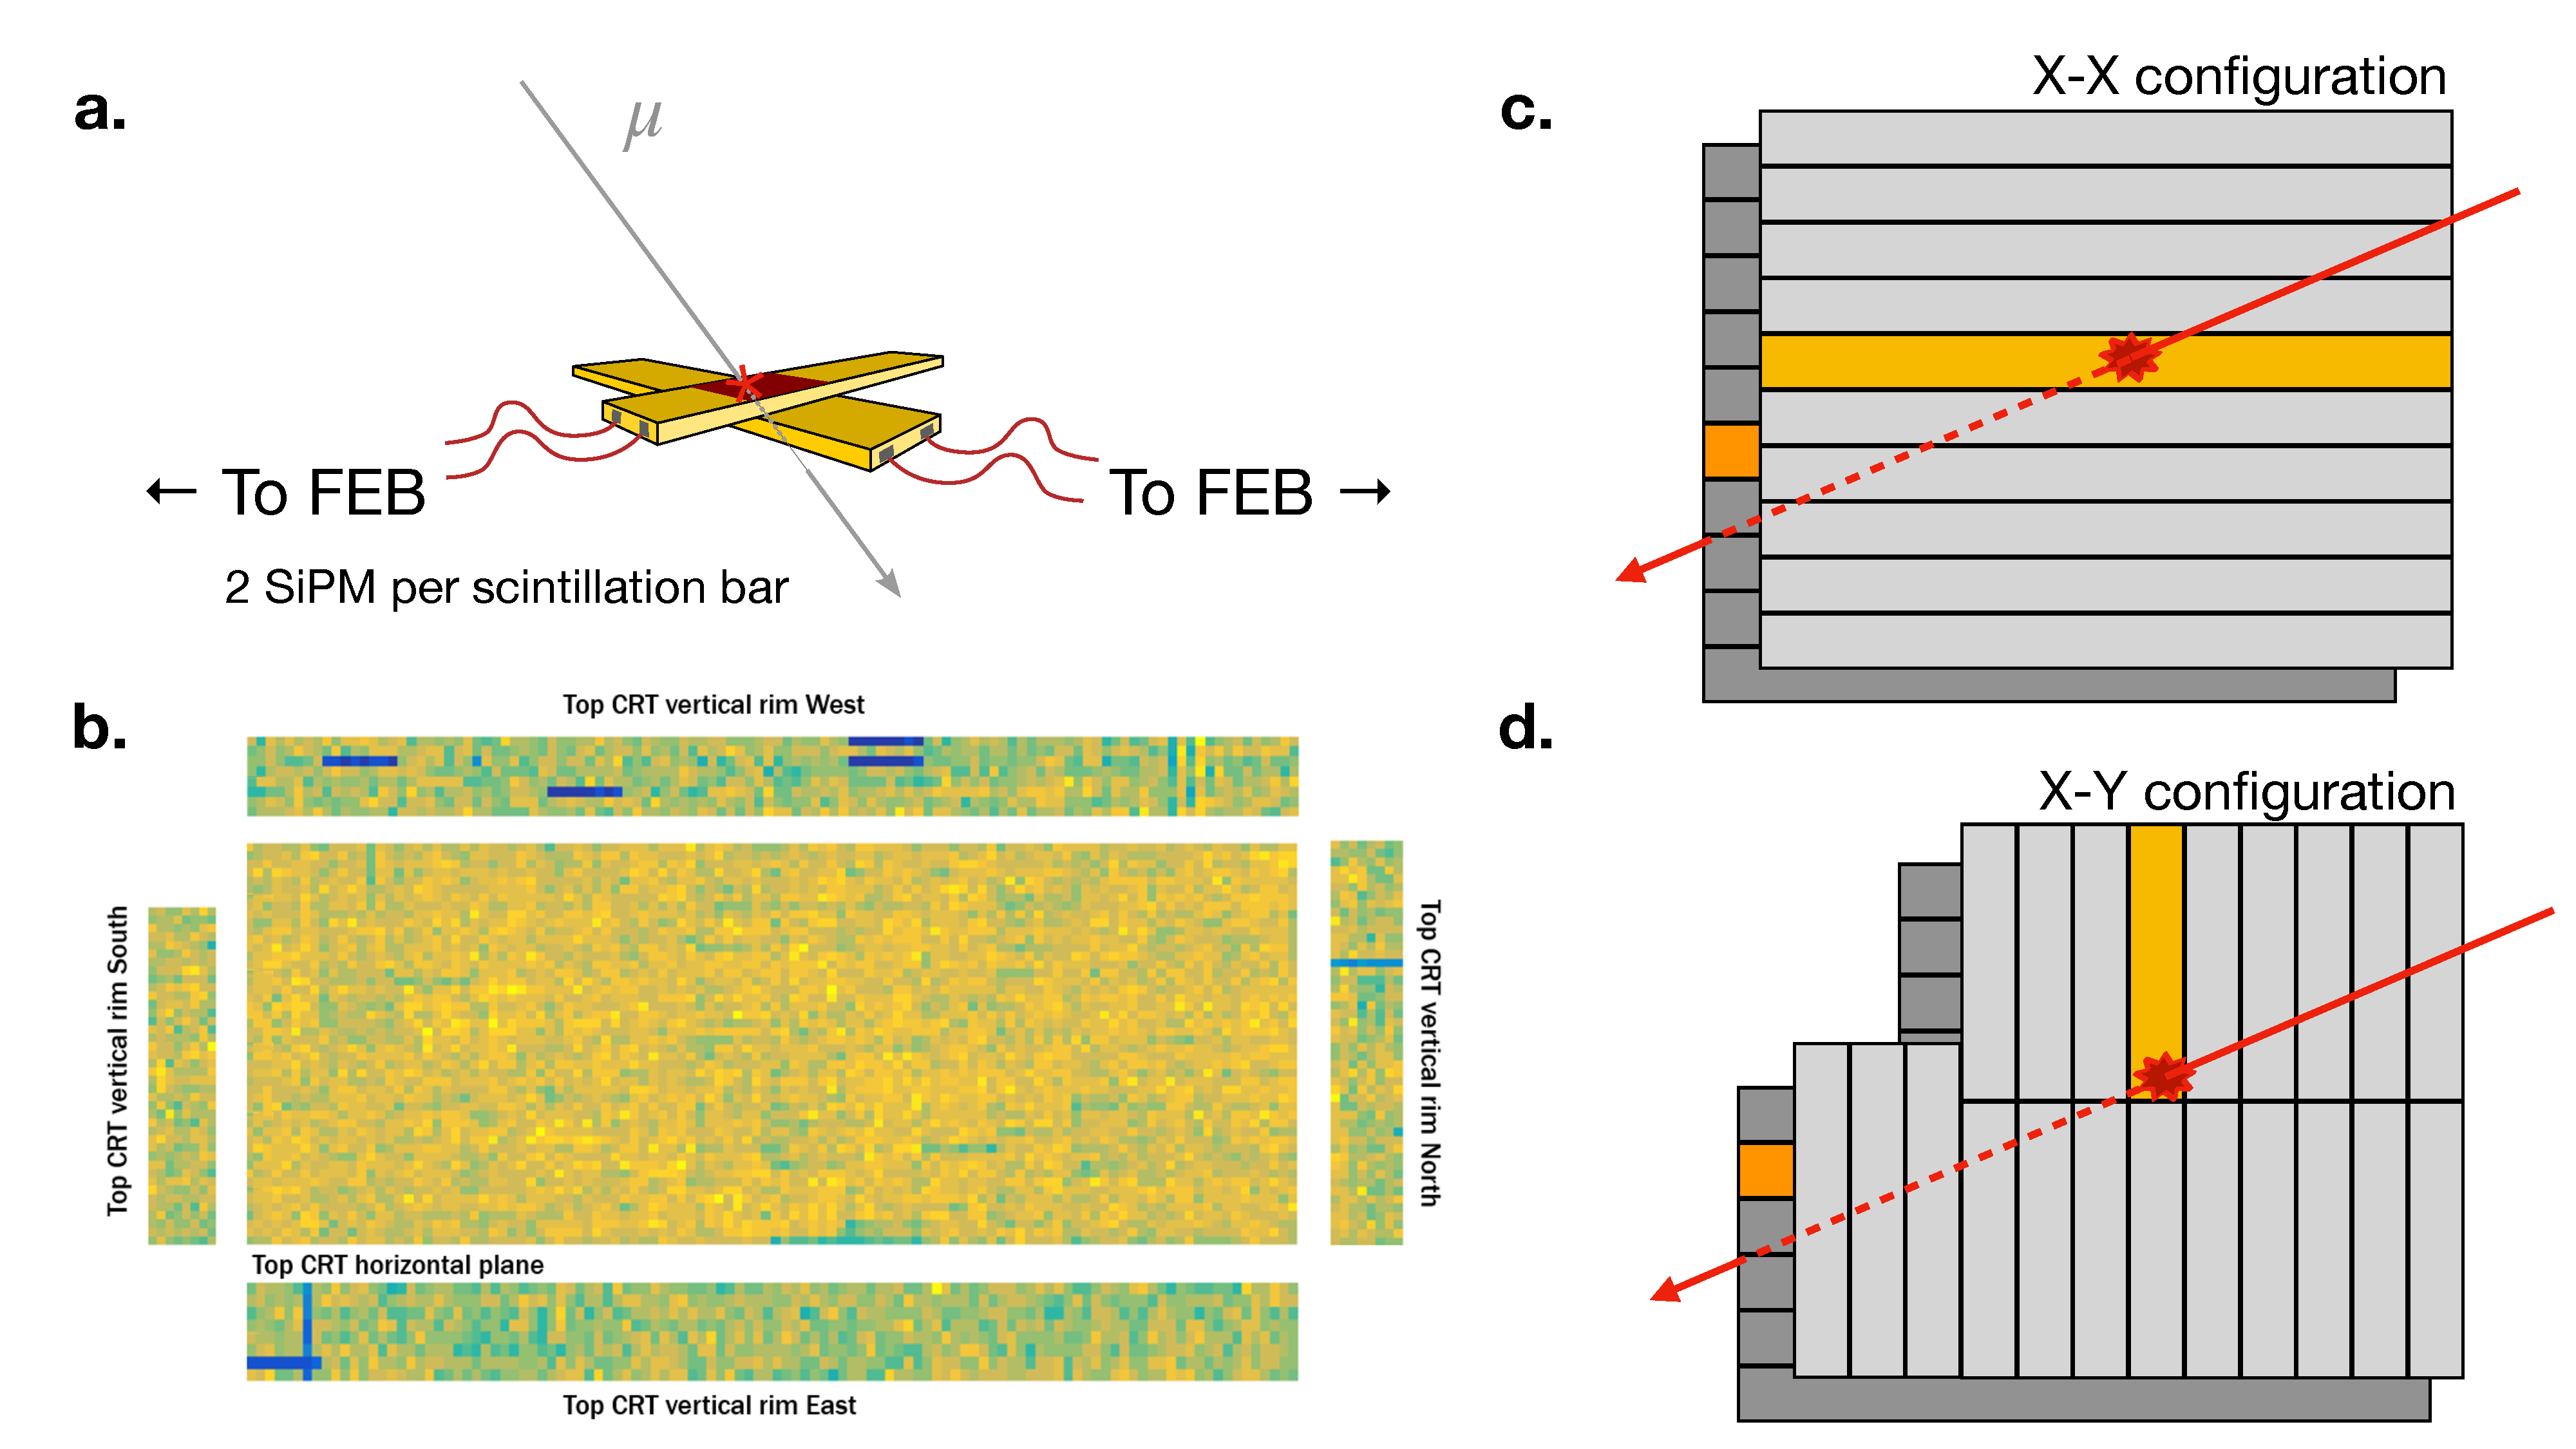
\includegraphics[width=\linewidth]{detector/CRT_all.pdf}
    \caption[CRT Hit reconstruction in space]{Illustration of CRT hit reconstruction position. (a) shows the reconstruction for the top CRT modules, where the coincidence between two scintillation bars is required. (b) shows the distribution of the CRT hits reconstructed in the different regions of the Top CRT. Blue regions
correspond to malfunctioning channels. (b) is taken from \cite{Poppi:2023zmp}, (a), (c) and (d) are adapted from \cite{arteroponsStudyReconstructionNuMuCC}.}
    \label{fig:CRT_reco}
\end{figure}

By exploiting the quadruple coincidence, the top CRT hits local position in each module with a known granularity of \qtyproduct[product-units=power]{23x23}{\cm}. A transformation is all that is required to know the hit position with respect to the ICARUS detector frame of reference. \autoref{fig:CRT_reco}b shows the distribution of the CRT hits using a collected calibration run. 

For the side CRT modules the reconstruction is slightly different. The coincidence of adjacent layers is reconstructed offline at the software level, due to the same modules being read by multiple FEBs. Hit scintillator strips are identified by selecting in each FEB the channel that generated the FEB trigger signal, which is the one with the highest charge amplitude. \autoref{fig:CRT_reco}c and d show two of the configurations of the CRT side module strips. The triggering strip is shown in yellow, and the red star shows the interaction point. The north, east and west side CRTs have the X-X configuration pictured in \autoref{fig:CRT_reco}c. For these, if two opposite SiPM signals are collected within \SI{150}{\ns}, and read out by two FEBs, the longitudinal position (across the strip) can be computed with respect to the centre position of the strip by comparing the $T_0$ timestamps recorded by each FEB, \begin{equation}
    z = \qty(T_B - T_A)/2 \cdot v_\mathrm{wls}, 
\end{equation} where $T_A$ and $T_B$ are, respectively, the two timestamps recorded by the FEBs, $z$ is the computed longitudinal position, and $v_\mathrm{wls}$ is the group velocity of the light signal inside the wavelength shifter fibre. The south CRT wall is using the X-Y configuration shown in \autoref{fig:CRT_reco}d, for which a software coincidence similar to that of the top wall is performed, exploiting the orthogonal relative position of the outer and the inner strips. 

The last step performed in \emph{Stage0} concerns the temporal matching of the light and CRT information. This step is crucial, especially for higher-level processing, where it can be exploited to improve the efficiency by which correct interactions are selected inside the detector, rejecting out-of-time activity using the CRT-PMT match. 

\section{TPC event reconstruction} \label{sec:TPC_reco_gen}

\emph{Stage1} is almost completely dedicated to performing the high-level event reconstruction, taking the \emph{Hit} objects created by the modules of \emph{Stage0} and transforming them to build the full interaction picture. This part of the event reconstruction interests primarily the TPC and PMT sub-detectors, since it is expected for most neutrino interactions to be contained inside the LAr volume, hence not to have any relation to CRT hits. 

To perform the event reconstruction inside the TPC, the starting point is given by the three collections of 2D hits created in \emph{Stage0}. Although new particle identification frameworks are constantly being developed for LArTPCs (one actively being developed in the context of the ICARUS reconstruction; see \autoref{sec:SPINE}), the Pandora Software Development Kit \cite{MicroBooNE:2017xvs} (henceforth called just Pandora) has been a constant baseline. The Pandora reconstruction chain takes the three 2D hits produced by the hit-finding algorithm as input, performing a topological reconstruction of the objects taking part in the interaction to reconstruct the energy deposits of each one. It specifically promotes the idea of a multi-algorithm approach to solving pattern-recognition problems. In this approach, the input building blocks (hits) describing the pattern recognition problem are considered by large numbers of decoupled algorithms. Each algorithm targets a specific event topology and controls operations such as collecting hits together in clusters, merging or splitting clusters, or collecting clusters in order to build a representation of particles in the detector. Each algorithm aims only to perform pattern-recognition operations when it is deemed ``safe'', leaving complex topologies to later algorithms. In this way, the algorithms can remain decoupled, and there is little inter-algorithm tension. Some algorithms are complex, whilst others are simple. The algorithms gradually build up a picture of the underlying events and collectively provide a robust reconstruction.
 
The hit-finding algorithm, providing the collections of 2D hits, is optimised to prefer efficiency over purity, reaching an efficiency greater than \SI{99}{\percent}; this might, however, lead to the creation of non-physical hits, especially in very noisy regions, that might cause failures in the pattern recognition steps. To prevent such problems, the collection of 2D hits produced by the hitfinding algorithm are filtered using the \emph{Cluster3D} algorithm. It runs over the set of wires of the three planes and, taking advantage of the fact that the $x$ coordinate --- the drift direction, or the waveform time coordinate --- is common across the planes, tries to look for time-correlated hits across the three planes. If matches are not found, or hits are isolated, then they are filtered out. The resulting filtered collection of hits is used as the input for the Pandora topological reconstruction. 

\subsection{Geometry of the ICARUS detector}

The Pandora reconstruction --- as any reconstruction paradigm for LArTPC would do --- heavily exploits the geometrical characteristic of the detector. Newer LArTPC detectors employ a common geometry to make it effortless to transition the software codebase from one to another. Being the first of its kind and being born with physics goals that extend beyond what are the physics goals of current LArTPC detectors, the ICARUS detector TPC geometry is unique. As already mentioned in \autoref{sec:ICARUS_T600}, and illustrated in \autoref{fig:i2_c_planes_wirepitch_detail}, ICARUS wire planes have some peculiarities. First, the wire orientation is different: it is common for TPC wires to be orientated \SI{+-60}{\degree} with respect to the vertical direction for the first two induction planes ($u$/$v$), and have the collection ($w$) plane wires vertical, whereas in the ICARUS detector the first induction plane features horizontal wires, and the second induction and collection planes are oriented \SI{+-60}{\degree}. This difference in wire orientation also requires the T300 modules of the ICARUS detector to have its planes split along the $z$ coordinate to avoid having \SI{18}{\meter} long wires, but at its maximum have \SI{9}{\meter} of wires. 

The geometrical parameter that is core for the Pandora software when performing the 3D reconstruction of the wire planes 2D projections is the angle at which the wire planes are orientated. This information is used to perform the spatial reconstruction of the hits collected in the different planes, using projective geometry. In Pandora each plane is called a view, and to each view is associated the angle at which the wires are orientated. In most LArTPCs the mapping between views and planes is univocal. For example, considering the SBND APA, both East and West APAs feature the $u$ plane at $+\SI{60}{\degree}$, the $v$ plane at $-\SI{60}{\degree}$ and the $w$ plane at \SI{0}{\degree} with respect to the vertical direction. In the ICARUS TPC, however, the requirement to have the induction-2 and collection plane's wire angle orientated in the same direction if seen in the drifting direction (see, for reference, \autoref{fig:i2_c_planes_wirepitch_detail}) means that the mapping is not unique and depends on which TPC of each T300 module is being considered. This has no apparent drawbacks, but there are some subtleties that have to be considered. For instance, the collection plane is often used, being the plane with the highest signal-to-noise ratio, to get a better evaluation of the deposited charge. The Pandora tools, under the assumption that the collection plane corresponds to the $w$ view, often just refer to it as the ``best plane'' (see for example, when computing the charge deposition variables used in the track identification BDT algorithm): this has recently been fixed with a workaround, but the same issue can be affecting the reconstruction performances in other algorithms. 

\subsection{Pandora approach to the event reconstruction} 

As already mentioned, Pandora takes an innovative approach to the topological event reconstruction, splitting the problem of pattern recognition into smaller, decoupled algorithms. The Pandora framework is well integrated inside the \emph{LArSoft} ecosystem and accessed via the \emph{LArPandora} translation module. This module handles the conversion from the \emph{LArSoft} Event Data Model (EDM) to the PAndora EDM, then initiates and applies the Pandora algorithms, and finally reconverts back from the Pandora EDM to the LArSoft EDM. The ICARUS detector consists of two separated T300 modules; thus, two parallel instances of the Pandora reconstruction are run on each event, corresponding to the east and west cryostats. Each Pandora instance runs the full list of algorithms on the corresponding T300 module. 

The inputs, translated from the LArSoft EDM to the Pandora EDM, are the collections of 2D hits in the $x$--wire plane, with $x$ representing the drift time and the second coordinate being the wire number. The $x$ coordinate is common across the views and thus is exploited to match the hits from different planes. The output of the pattern recognition algorithms are the Particle Flow Particles, or PFParticles, objects; each PFParticle correspond to a distinct track or shower, and it is associated with a list of 2D clusters, which are groups of hits on the same planes belonging to the same reconstructed object. Each PFParticle is also associated with a set of 3D positions (named SpacePoints) and with a vertex position, defining its interaction point or its first energy deposition. PFParticles are finally arranged in a hierarchy, which identifies parent-daughter relationships. For each interaction defined as neutrino-like, one empty PFParticle is created, identifying the neutrino PFParticle, and is associated with the primary interaction vertex. \autoref{fig:LArPandora_dependencies} shows all data products produced by the Pandora translation into LArSoft EDM and their interdependency. 

\begin{figure}
    \centering
    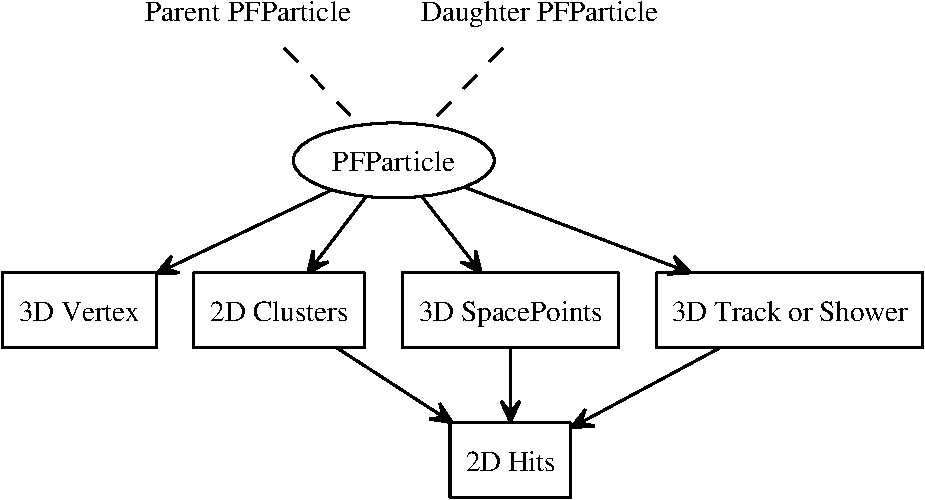
\includegraphics[width=0.75\linewidth]{pandora/LArSoftOutput.pdf}
    \caption[LArPandora output data products]{The Pandora output data products, as persisted in the LArSoft Event Data Model. Navigation along PFParticle hierarchies is achieved using the PFParticle interface, represented by dashed lines. Navigation from PFParticles to their associated objects is represented by solid arrows. Taken from \cite{MicroBooNE:2017xvs}. }
    \label{fig:LArPandora_dependencies}
\end{figure}

Three Pandora multi-algorithm reconstruction paths have been created for use in the analysis of ICARUS data: PandoraFastReco, PandoraCosmic and PandoraNeutrino. The last two are, as the names suggest, aimed at the reconstruction of precise interaction topologies; namely,  PandoraCosmic is optimised for the reconstruction of cosmic-ray muons and their daughter delta-rays, whereas PandoraNeutrino is optimised for the reconstruction of neutrino interactions. The PandoraFastReco path is run prior to both PandoraNeutrino and PandoraCosmic, with the precise aim of identifying \emph{unambiguous} cosmic-ray muons, employing a faster reconstruction pipeline. The output of the PandraFastReco path corresponds to a list of candidate cosmic rays. This list is then examined by a tagging module which identifies unambiguous cosmic-ray muons, based on their topological features, and removes their hits from the list. This allows for a higher signal-to-noise ratio and a better topological reconstruction in the subsequent steps. \autoref{fig:pandora} illustrate the subsequent steps applied to each event by the Pandora reconstruction. 

\begin{figure}
    \centering
    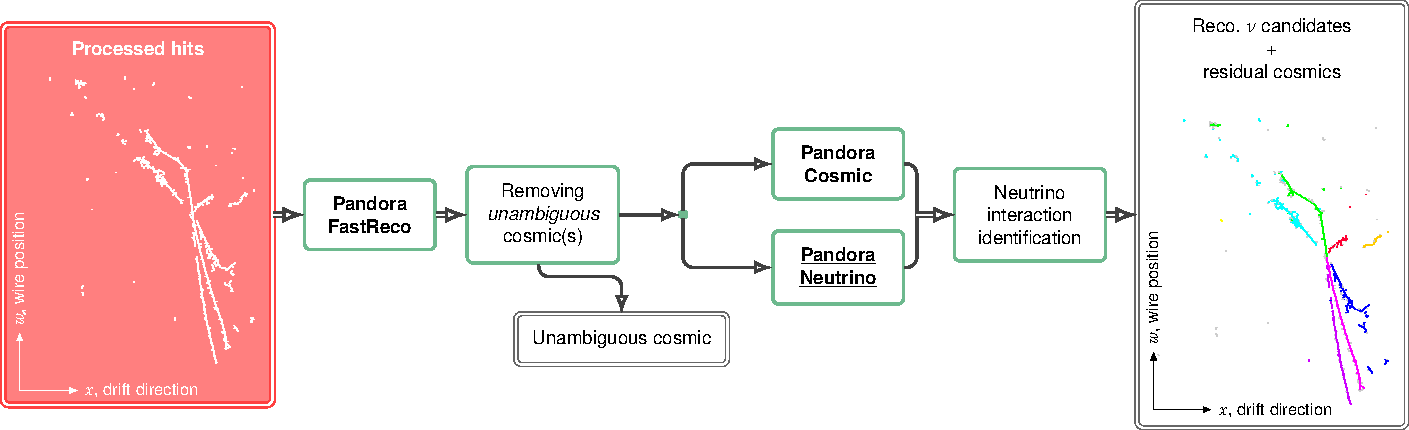
\includegraphics[width=\linewidth]{pandora/figure_Pandora/pandora.pdf}
    \caption[Overview of the Pandora reconstruction chain]{Illustration of the Pandora reconstruction chain. Starting from a set of image-like collections of 2D hits, as shown in the left red panel, the Pandora approach is to first address a fast and rough reconstruction, aimed at removing the particles that are clearly cosmic-ray muons. Then each interaction inside the detector is passed through both PandoraCosmic and PandoraNeutrino chains to refine their reconstruction. }
    \label{fig:pandora}
\end{figure}

\subsection{PandoraFastReco: \emph{unambiguous} cosmic hits removal} \label{sec:fast_reco}

The first Pandora path applied to the events consists of a set of tools aimed at performing a \emph{draft} reconstruction of all hits identified during the readout window, providing a list of ``unambiguous'' cosmic-ray particle candidates. The PandoraFastReco shares most of the algorithms with the PandoraCosmic reconstruction path, since they both aim at reconstructing interactions characterised by a long straight track, usually crossing the full detector volume. The path, illustrated in \autoref{fig:PandoraFastReco} is composed of four main stages. 

\begin{figure}
    \centering
    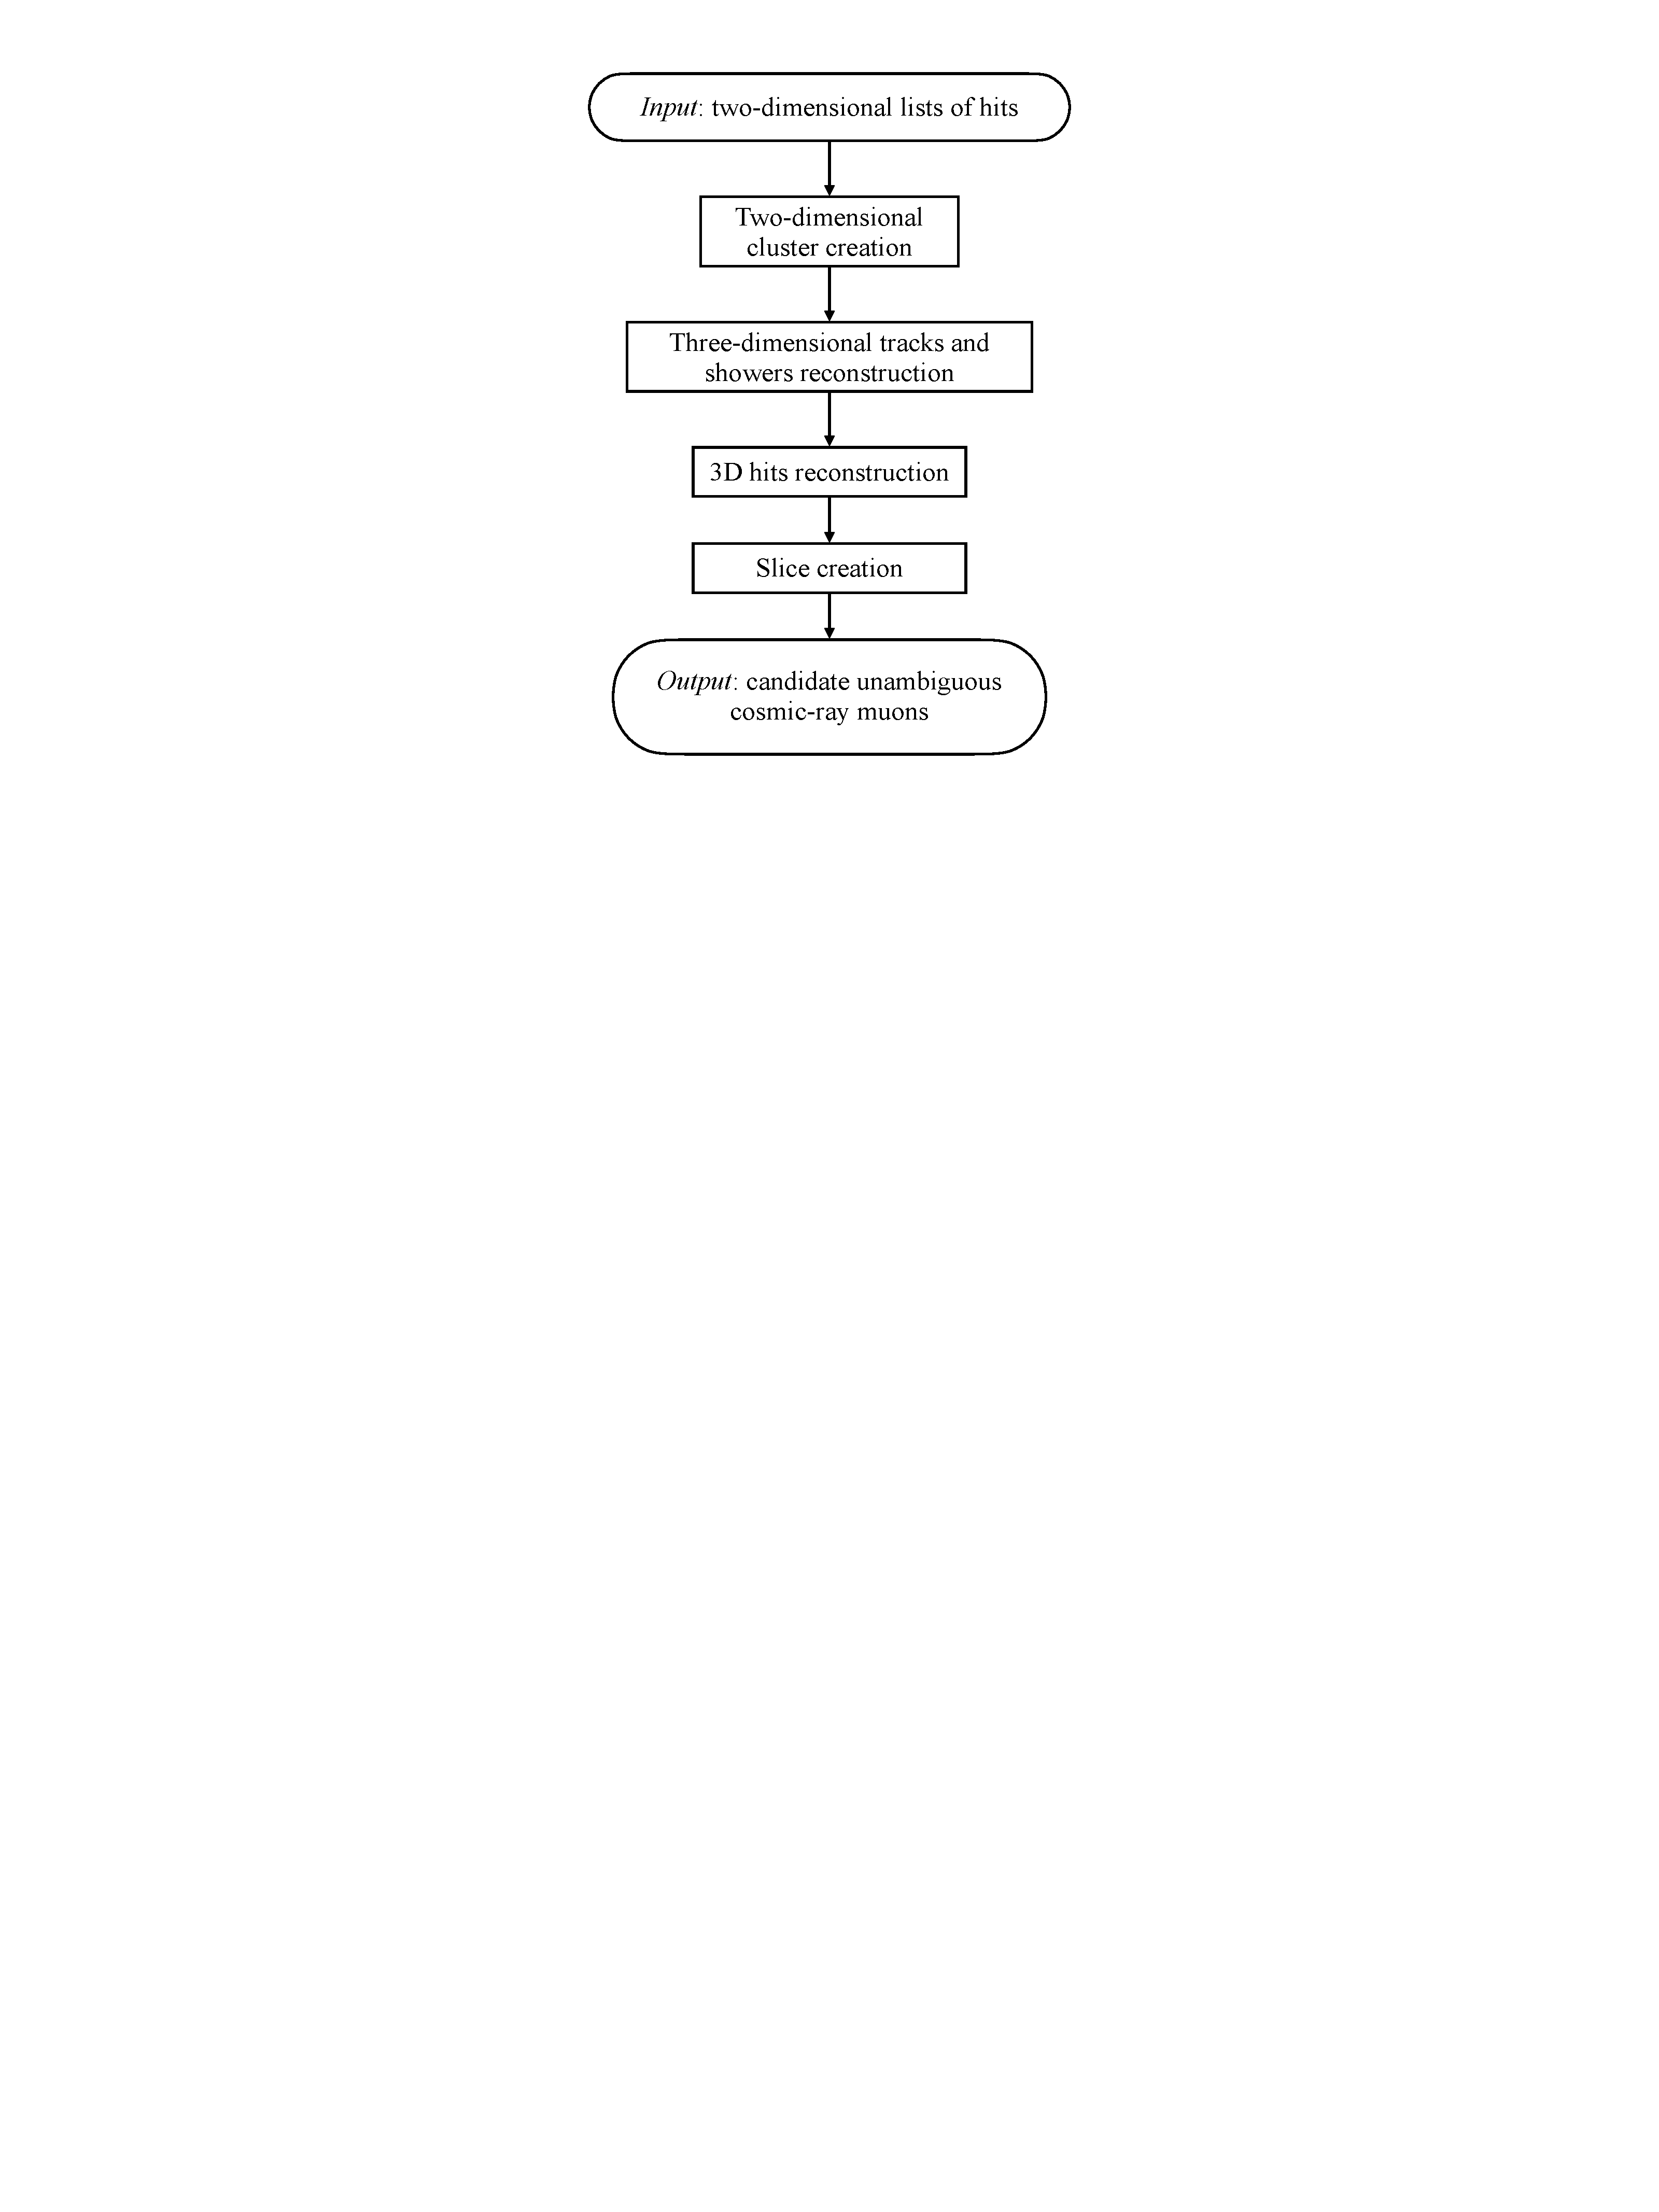
\includegraphics[width=0.5\linewidth,trim={16cm 47cm 16cm 1.5cm}, clip,page=1]{pandora/Pandora.pdf}
    \caption[PandoraFastReco path illustration]{Illustration of the main steps of the PandoraFastReco path, which is applied as a first ``draft reconstruction''. This path aims at creating unambiguous cosmic-ray muon candidates that are then flagged and whose hits are removed. Adapted from \cite{MicroBooNE:2017xvs}}
    \label{fig:PandoraFastReco}
\end{figure}

\subsubsection{Two-dimensional reconstruction}

The first step takes as input the three separate lists of two-dimensional hits, corresponding to the three views or wire planes. For each, the TrackClusterCreation algorithm creates bidimensional clusters of hits, representing continuous lines of hits. Bifurcations, kinks or any topological branch feature stop the creation of a cluster and start the creation of another cluster. This approach ensures that initial clusters have high purity, meaning a high number of correctly associated hits, but a lower completeness, meaning that a single true particle is split into multiple clusters. At this point, cluster-merging algorithms identify associations between multiple 2D algorithms, improving the track completeness without affecting its purity. Additionally, algorithms are present to stitch together clusters that are split due to unresponsive wires or hits under the reconstruction threshold (that are not reconstructed). 

To improve purity, cluster splitting algorithms refine the selection by breaking simple clusters if topological features indicate that there are ``spurious'' hits inside the cluster. 

\subsubsection{Three-dimensional reconstruction}

After 2D clusters are created, they are collected together with the aim of creating groups of 2D clusters that represent the same individual track particle. The challenge these algorithms need to address is to identify consistent groupings of clusters from the different views. The 3D track reconstruction is performed by three main algorithms: the ThreeDTransverseTracks algorithm, the ThreeDLongitudinalTracks algorithm and the ThreeDTrackFragments. The former does, however, do most of the work. 

The ThreeDTransverseTracks algorithm identifies all the suitable combinations of clusters from the three readout planes and inspects these combinations to identify cluster-matching ambiguities. Those ambiguities are used to iteratively improve on the 2D cluster and remove the ambiguities. In this way, the matching becomes \emph{unambiguous}. The groupings of three clusters from the three readout planes are created by exploiting the common $x$ drift coordinate. On each view sliding fits are performed on the clusters; given a point on the $x$ coordinate, then the position of the sliding fit on two of the three views can be extracted, for example, the position on the $u$ and $v$ views. These positions, together with the coordinate transformation plugin, can be used to predict the position of the third cluster --- in the example, in the $w$ view --- at the same $x$ drift coordinate. This prediction can be compared to the sliding fit position on the third view, and the same can be done with all possible combinations --- $u,v\to w$; $v,w\to u$ and $w, u \to v$. By performing such fits, and therefore checking the possible groupings of clusters across the three views, connections between them are created. The goal is to make these connections unambiguous, i.e. no two unique clusters from the same view are grouped together. As described in \cite{MicroBooNE:2017xvs}, multiple tools query the different connection types across the views. Once no ambiguities are observed in the sets of clusters, the algorithm passes a list of sets of two (or three) clusters from different views to the following algorithms. Examples of the operation of these tools is illustrated in \autoref{fig:PandoraThreeDTracks}. 

\begin{figure}
    \centering
    \subfloat[]{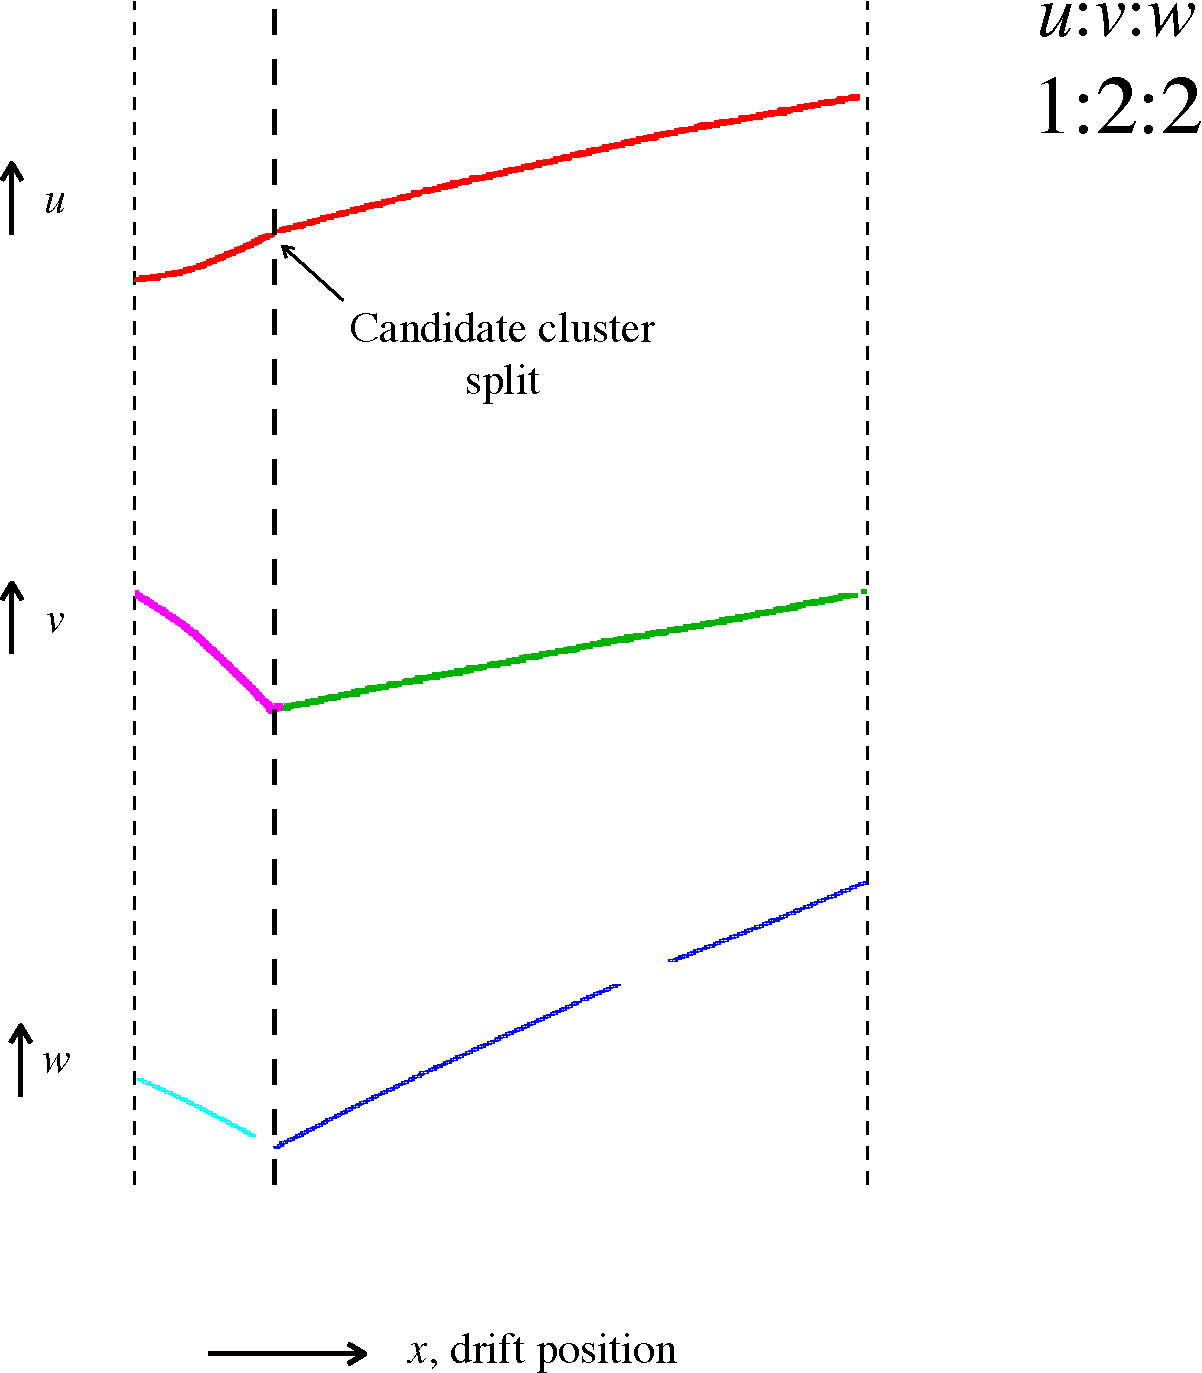
\includegraphics[width=0.5\linewidth]{pandora/ThreeDTracksTools/OvershootTracksTool.pdf}\label{fig:OvershootTracksTool}}
    \subfloat[]{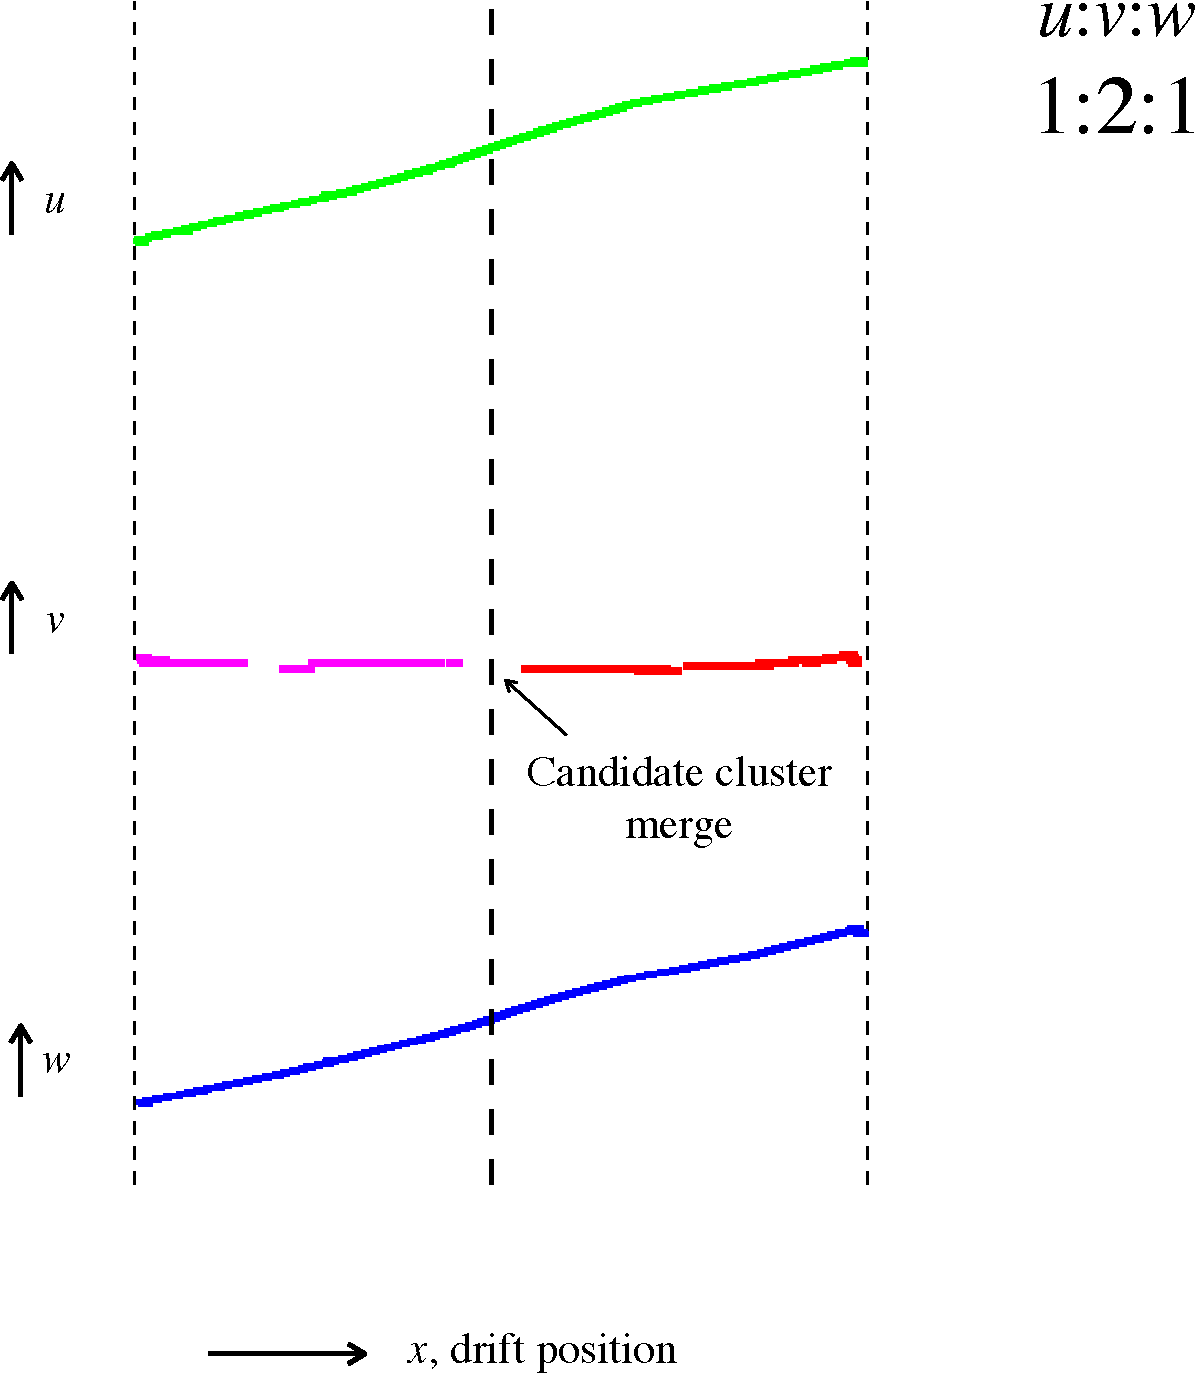
\includegraphics[width=0.5\linewidth]{pandora/ThreeDTracksTools/UndershootTracksTool.pdf}\label{fig:UndershootTracksTool}}
    \caption[Three-dimensional reconstruction helper tools]{Example of two of the tools querying the 2D clusters' connections. \ref{sub@fig:OvershootTracksTool} aims at resolving the ambiguities that arise from one view having two clusters merged into one. This ambiguity is resolved by splitting the cluster with the information from the other two views. \ref{sub@fig:UndershootTracksTool} is diametrically opposed to the former, in the sense that it tries to merge one cluster that was split in half in the previous steps. }
    \label{fig:PandoraThreeDTracks}
\end{figure}

\subsubsection{Three-dimensional hit reconstruction}

At this point, the assignment of hits to reconstructed particles is complete, each particle containing hits from one, two or usually three views. For each 2D hit a 3D point is created, with multiple approaches depending on the cluster topology. In both cases, the common section is the minimisation of a $\chi^2$-like value to get the best $y,z$ values by fixing a certain $x$ coordinate. 

After the 3D hit creation, candidate muon cosmic-ray particles are created, and they are tagged to filter out hits belonging to the unambiguously cosmic-ray particles. Ambiguous hits are passed to subsequent paths of the reconstruction, namely PandoraCosmic and PandoraNeutrino. 

\subsection{PandoraNeutrino: topological neutrino event reconstruction} \label{sec:PandoraNeutrino}

A key requirement for the PandoraNeutrino reconstruction path is that it should be able to deal with the presence of cosmic-ray muon remnants. The approach to address this problem is therefore to run the same 2D clustering, 3D cluster matching and 3D hit reconstruction described in \autoref{sec:fast_reco}. This is actually the second purpose of the PandoraFastReco path. After this path is run, 3D hits are divided into \emph{slices}, which are separate lists of hits, using proximity-based metrics. The idea is to isolate neutrino interaction and cosmic-ray interaction in different slices. The original 2D hits associated with each slice are then used as an input to the dedicated neutrino reconstruction, which is described in this section. 

The PandoraNeutrino dedicated reconstruction (shown in its entirety in Figure \ref{fig:PandoraNeutrino}) begins with a track-orientated clustering algorithm and a series of topological algorithms. Before processing the 2D clusters, the interaction vertex is reconstructed. 

\begin{figure}
    \centering
    \subfloat[]{\includegraphics[width=0.5\linewidth,trim={16cm 41cm 16cm 1.5cm}, clip,page=2]{pandora/Pandora.pdf}\label{fig:PandoraCosmic}}
    \subfloat[]{\includegraphics[width=0.5\linewidth,trim={16cm 40cm 16cm 1.5cm}, clip,page=3]{pandora/Pandora.pdf}\label{fig:PandoraNeutrino}}
    \caption[PandoraCosmic and PandoraNeutrino paths illustration]{\ref{sub@fig:PandoraCosmic} illustrated the PandoraCosmic path, applied after the first draft pass, parallel to the neutrino path. \ref{sub@fig:PandoraNeutrino} illustration of the PandoraNeutrino steps, applied to each slice in the event. Adapted from \cite{MicroBooNE:2017xvs}}
    \label{fig:PandoraCosmicNeutrino}
\end{figure}

\subsubsection{Three-dimensional vertex reconstruction}

The reconstruction of the neutrino interaction vertex proceed via two steps. Firstly, the CandidateVertexCreation algorithm creates a list of possible vertices. Comparing pairs of 2D clusters, ensuring that the two 2D clusters are from different views and have some overlap in the $x$ coordinate, the algorithm creates up to four neutrino vertices candidates for each 2D clusters pair, one for each endpoint of the 2D clusters. 

After the identification of the candidate neutrino vertices, it is necessary to identify the most probable vertex candidate. This is archived by using a BDT algorithm, which assigns each vertex a score. The vertex candidate with the highest score is finally selected to be the correct neutrino interaction vertex. 

The variables used to perform the classification and identify the most suitable vertex candidate include both properties of the reconstructed event and features of the candidate vertices. The former variables include the total number of hits, clusters and vertex candidates associated to the event; the fraction of hits likely originating from a shower based on cluster length and true associated particle; an estimate of the energy and of the area of the event, extracted from the total clusters span along $x$ and $z$ directions; and an estimate of how longitudinal the event is with respect to the beam direction. 

This is the first of the two ``machine-learning''-like currently used algorithms in the Pandora-based event reconstruction for the ICARUS detector. 

\subsubsection{Three-dimensional track and shower reconstruction}

The PandoraNeutrino reconstruction, after the vertex creation stage, proceeds to reconstruct the three-dimensional tracks in the same way as described in previous sections. PandoraNeutrino, however, attempts also to reconstruct primary electromagnetic showers, arising from electrons and photons interacting in LAr. 

Using a set of topological cuts, 2D clusters are classified either as track-like or shower-like. Existing track particles that are now deemed to be shower-like are dissolved, to allow assessment of the cluster as shower candidates. At this point, on each view clusters representing shower branches candidates are merged. Showers are grown from the candidate shower spines adding shower branches where association is plausible. 

Following the 2D shower reconstruction, the ThreeDShowers algorithm builds the 3D hits in a similar way to how 3D hits were built for the track-like particles, as described before. 

After the 3D showers are finally built, a second pass of the 3D track reconstruction is applied to recover any inefficiencies associated with dissolving track particles to examine their potential as showers. Once both 3D tracks and 3D showers are consolidated, particle refinement algorithms try to improve on both hit completeness and purity, dissolving unassociated 2D clusters or, especially in the case of showers, adding 2D clusters that were left from previous steps of the reconstruction. 

\subsubsection{Particle hierarchy reconstruction}

After the 3D reconstruction has taken place, the nex step in the PandoraNeutrino reconstruction is to organise the reconstructed particles into a hierarchy. This follows some subsequent steps, namely \begin{itemize}
    \item The neutrino particle is created and associated with the 3D interaction vertex.
    \item The 3D particles deemed to be associated with the interaction vertex are added as primary daughters of the neutrino particle.
    \item Algorithm tools look to add subsequent daughter particles to the existing primary daughter of the neutrino --- for example, the decay electron might be added to a primary muon particle. 
    \item 3D vertex position (endpoints) are calculated for each of the particles in the neutrino hierarchy. This is the neutrino interaction vertex for primary particles, and the point of closest approach to their parents for secondaries
\end{itemize}

The last step of the PandoraNeutrino reconstruction handles the classification, by means of a BDT algorithm, of reconstructed particles as tracks or showers. The classification is performed on a set of topological and calorimetric variables. A detailed description of the variables, the training process and the classification efficiency is discussed in \autoref{chap:mva_internship}, as part of the work performed during an internship at Fermilab. 

\subsection{PandoraCosmic: cosmic-ray muon reconstruction}

Parallel to the neutrino-interaction reconstruction path, PandoraNeutrino, the PandoraCosmic path is also run, on the same set of hits, with the precise aim to reconstruct the remaining cosmic-ray interactions with greater detail. 

The PandoraCosmic path is very similar to the PandoraFastReco path since it aims as well at the reconstruction of clear cosmic-ray muon particles. The only differences are the lack of the slice creation step, unique to the PandoraFastReco path, and the addition of the delta-ray reconstruction stage. The path is clearly illustrated in Figure \ref{fig:PandoraCosmic}. 

\subsubsection{Delta-ray reconstruction}

Unique to the PandoraCosmic path, before actually performing the creation of the 3D position inside the detector volume (see, for reference, Figure \ref{fig:PandoraCosmic}), a delta-ray reconstruction step dissolves any 2D clusters that have not been assigned to any reconstructed particle. The assumption for these algorithms is that these clusters likely represent fragments of delta-ray showers. Once 2D clusters are created, the between-views match is performed primarily exploiting the common $x$ coordinate. Parent cosmic ray particles are identified via comparisons of intra-cluster distances. 

\section{Calorimetry and particle identification} 

Following the topological event reconstruction performed by the Pandora algorithm, calorimetric information is computed with the use of multiple LArSoft modules. 

Once 3D trajectories, made of 3D space-points, have been reconstructed, using the relevant quantities associated with the hits --- hit area, hit time, and the track pitch lenght --- the aim is to be able to reconstruct the energy loss, $\dv*{E}{x}$, which is core to the  subsequent particle identification. The energy loss is computed for each hit from the $\dv*{Q}{x}$, expressed in ADC counts per centimetre. This is obtained, in turn, by the ratio of the area under the hit ($\dd Q$) and the track pitch ($\dd x$), which is computed from the direction of the track, knowing that the wire pitch for the ICARUS detector is of \SI{3}{\mm}, $\dd x = \SI{3}{\mm}/\cos\gamma$, where $\gamma$ is the three-dimensional angle between the local direction of the track and the wire direction. 

Calorimetry measurements require a good understanding of the charge response of the wires inside a LArTPC. The $\dv*{Q}{x}$ measured on the wires might substantially differ from the original $\dv*{Q}{x}$ at the location where the ionisation occurred; hence, it needs to be corrected before charge deposition is converted into energy loss. The process of removing these charge response effects takes the name of ``charge equalisation''. This process happens in three parts: \begin{inparaenum}
    \item charge equalisation in the drift direction $x$;
    \item the equalisation on the wireplane direction $y$ and $z$; and 
    \item the equalisation across the four TPCs in the ICARUS detector. 
\end{inparaenum} Charge equalisation is performed using a cosmic off-beam dataset that crosses both the LAr volume and leaves a hit on the CRT panels. 

The main effects that affect the $\dv*{Q}{x}$ in the ICARUS detector are \begin{itemize}
    \item Argon impurities: when electron drift toward the anode, they can be captured by the electronegative impurities (mainly $\mathrm{O_2}$ and $\mathrm{H_2O}$). Since the electron attachment is modeled as an exponential decay, the measured $\dv*{Q}{x}$ is corrected as \begin{equation}
        \eval{\dv{Q}{x}}_\mathrm{corrected} = \eval{\dv{Q}{x}}_\mathrm{measured} \exp(\frac{t_\mathrm{hit}-t_0}{\tau}),
    \end{equation} where $\tau$ is the electron lifetime. The electron lifetime measured in the ICARUS detector range between \qtyrange{4}{8}{\ms}. 

    \item Drift field distortions: the ionisation process inside liquid argon, other than producing a plethora of free electrons, gives rise to Ar ions. Those contribute to disuniformities of the drift electric field. Additionally, the ICARUS cathode plane is not completely flat, and this also produces disuniformities of the field. 

    \item Diffusion: electrons do not drift in perfect linear paths to the anodes but get diffused by elastic interaction in LAr. 
\end{itemize} Details on what the individual steps are to correct these effects are given in \cite{arteroponsStudyReconstructionNuMuCC}. 

After the calibration steps, to convert the $\dv*{Q}{x}$ into a deposited energy value, we need to take into account the fraction of electrons that survive the recombination without ion, $\mathcal{R}$, the amount of energy it it required to ionise an argon atom, $W_\mathrm{ion} = \SI{23.6}{eV}$ and the electronic gain $\mathcal{G}$ that converts ADC counts into the number of drifted electrons collected on the readout planes. With these information, it is possible to compute the $\dv*{E}{x}$ like \begin{equation}
    \dv{E}{x} = \frac{W_\mathrm{ion}}{\mathcal{R\cdot G}} \dv{Q}{x}. 
\end{equation}

From the reconstructed energy deposition per centimetre, it is possible to compute the full deposited energy like \begin{equation}
    E = \sum_i^\mathrm{all\ hits} \qty(\dv{E}{x} )_i \cdot \dd x_i. 
\end{equation}

Using the calorimetric information, it is possible to develop a $\chi^2$-like score that helps us identify the particle species. The underlying assumption is that, if the particle stops inside the TPC active volume, the $\dv*{E}{x}$ energy loss versus the residual range\footnote{Residual range is defined as the distance of an energy deposition within a track from the track's endpoint.} is a powerful tool to distinguish charged particles. The PID score is defined, therefore, as \cite{arteroponsStudyReconstructionNuMuCC} \begin{equation}
    \mathrm{PID} = \chi^2/\mathrm{ndof} = \sum_\mathrm{hit} \qty(\frac{{\dv*{E}{x}}_\mathrm{measured} - {\dv*{E}{x}}_\mathrm{theory}}{\sigma_{\dv*{E}{x}}})^2 \Big/ n_\mathrm{hits}. \label{eq:PID}
\end{equation}

\section{SPINE: machine learning particle identification} \label{sec:SPINE}

This thesis focuses on developing tools for the event reconstruction process described above, which is referred to as ``Pandora event reconstruction'' within the collaboration. However, recent inroads in Computer Vision (CV) and Machine Learning (ML) have motivated a new approach to the analysis of particle imaging detector data. Additionally, having multiple different approaches to event reconstruction can be crucial in proving the robustness of each one. 

Inside the ICARUS collaboration, an effort to develop an ML-based end-to-end reconstruction chain started and has now reached a mature stage, at which the performances and the robustness of the tools allow for analyses to be performed. This approach, named SPINE (Scalable Particle Imaging with Neural Embedding), consists of a hierarchical set of neural networks that are optimisable end-to-end. 

A schematic representation of the SPINE framework is shown in \autoref{fig:SPINE}. 

The starting point for the reconstruction are the same three readout planes that are processed through the Cluster3D algorithm. The Cluster3D algorithm is used (see \autoref{sec:TPC_reco_gen}) as a hit filter but does actually perform a simil-3D reconstruction that is used as auxiliary input to the SPINE processing. The hits that come out of the Cluster3D algorithm are passed through a UResNet architecture that aims at removing the so-called ghost hits. These are 3D hits created by an incorrect combination of 2D hits. Filtered positions are referred to as ``deghosted'' 3D space points. 

\begin{figure}
    \centering
    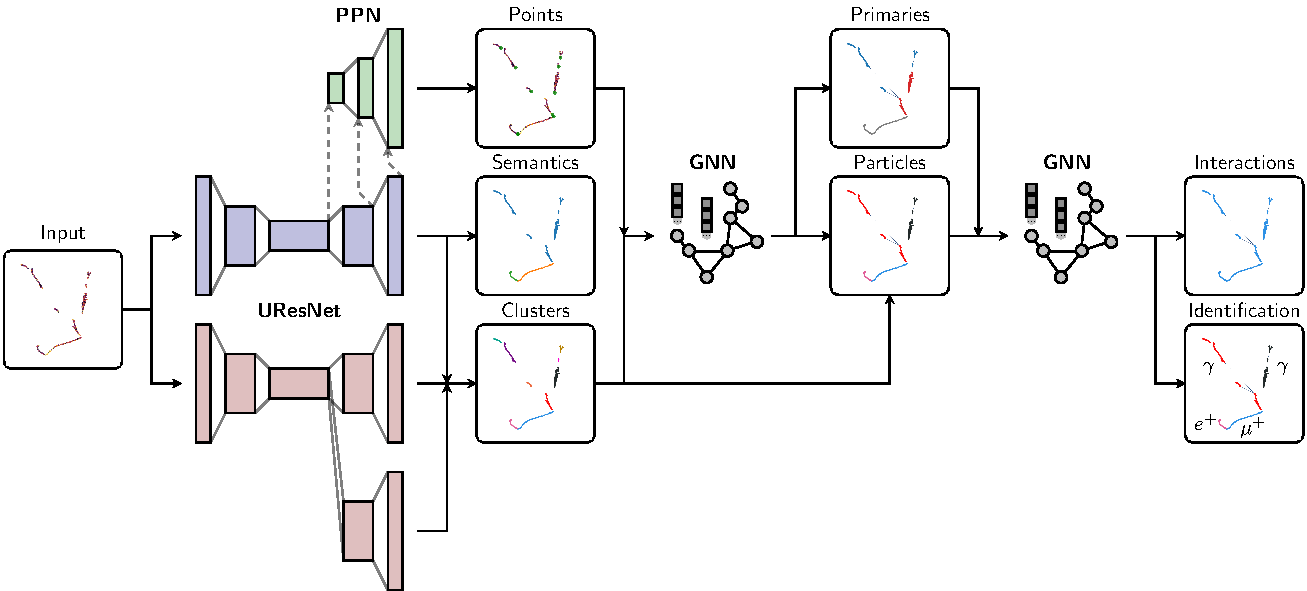
\includegraphics[width=\linewidth]{detector/mlreco_full_chain.pdf}
    \caption[SPINE end-to-end machine learning approach]{Schematic architecture of the end-to-end, ML-based reconstruction chain for LArTPCs. Taken from \cite{Drielsma:2021jdv}. }
    \label{fig:SPINE}
\end{figure}

The next step in the reconstruction chain is the classification of the deghosted 3D hits into categories based on the activity that produced them --- tracks, electromagnetic showers, Michel electrons, delta rays and low-energy depositions. This algorithm (shown in blue in \autoref{fig:SPINE}) uses the same UResNet architecture as the previous step. Parallel to this (shown in red in \autoref{fig:SPINE}) is a similar algorithm that aims at identifying and building dense particle clusters. The two outputs are aggregated and then passed as input to the next steps of the reconstruction. 


At this point of the SPINE reconstruction chain, groups of spacepoints corresponding to particle fragments have been identified, with semantic labels assigned to them. A Graph Neural Network aims then at clustering these groups of hits into particles. Two functionally identical GNNs are employed, called GrapPA-Track and GrapPA-Shower, targeting specific interaction topologies, namely tracks and showers. Details on the implementation and working of these algorithms are given in \cite{Drielsma:2021jdv}. 

The final stage of the SPINE reconstruction is to cluster particles into interactions. One interaction (the equivalent to the Pandora slice) is a collection of particles originating from the same interaction vertex. Particles directly associated with the interaction vertex are called primary particles, whereas other particles are labelled as secondaries. In addition to the interaction clustering, the network is also tasked with predicting the particle type (photon, electron, muon, proton, or pion; see \cite{DeepLearnPhysics:2020hut}). The architecture is still that of a GNN. The output of this network are all the interaction primary particles, each with a list of secondary particles, all with their types. 

\section{Simulation of the full detector}

\begin{figure}
    \centering
    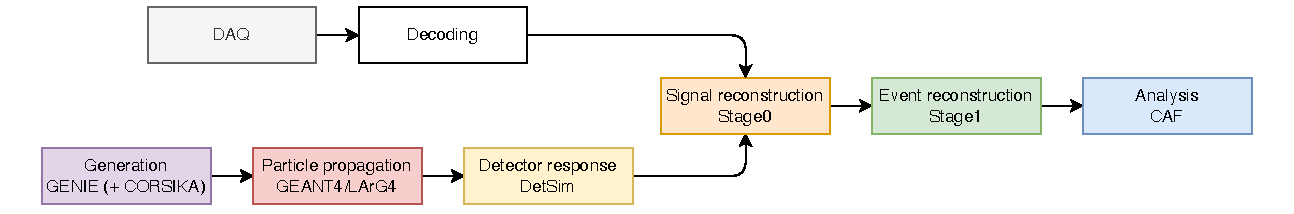
\includegraphics[width=\linewidth]{pandora/LArSoft_all.drawio.pdf}
    \caption[LArSoft complete overview]{Complete processing flow for both data and simulation, from the collection/simulation to the final analysis. }
    \label{fig:LArSoft_flow}
\end{figure}

The LArSoft framework that runs the full event reconstruction is also used to perform event simulation, from the generation of the interaction, performed using the GENIE Monte Carlo neutrino generator, to the particle passage, performed using the GEANT4 package, accessed through the LArG4 framework, to detector simulation, covering all the individual subsystems of the ICARUS detector. The output of the simulation is identical to the datastream collected by the detector and therefore can be used to perform Monte Carlo studies on the reconstruction pipeline. Details of the full event simulation are in \cite{arteroponsStudyReconstructionNuMuCC}, and \autoref{fig:LArSoft_flow} shows a full overview of the flow data product and simulations follow within the LArSoft infrastructure.